\chapter{Sistemi di equazioni lineari e matrici}
\label{chap:eqlinematrici}

Per definire rigorosamente cosa si intenda per equazione lineare
(o equazione di $1^o$ grado) e scrivere il generico esempio di
equazione lineare, si trova prima una notazione conveniente per
denotare tali equazioni.\\
Infatti, per non avere limitazioni sul numero delle incognite,
non è possibile continuare a indicarle con le lettere
dell'alfabeto $x,y,z,etc.$, che sono in numero limitato, ma
verrà utilizzata sempre la stessa lettera, tradizionalmente
la $x$ con degli indicatori numerici che consentono di
quale incognita si tratta: $x_1,x_2,\dots,x_n$ con, dove $n$ è
un numero naturale. Facendo un esempio di strutturate in questo
modo, si otterrà una situazione di questo tipo
\begin{equation}
  \label{eq:eqlinematrici1}
  a_1x_1+a_2x_2+\cdots+a_nx_n=b
\end{equation}
dove $b,a_1,a_2,\dots,a_n$ sono elementi di un campo
(solitamente, il campo dei numeri reali o quello dei complessi)
che svolgono il ruolo rispettivamente di termine noto e
coefficienti delle incognite (per ogni incognita $x_i$, bisogna
denotare il suo coefficiente con una lettera, $a_i$ con lo stesso
indice dell'incognita).\\
Dare una soluzione dell'equazione (\ref{eq:eqlinematrici1})
significa trovare degli elementi del campo, ovvero dei numeri,
che sostituiti alle incognite rendano l'ugualianza vera.\\
Ad esempio, nell'equazione lineare in due incognite $x_1-x_2=1$
a coefficienti nel campo dei reali $\mathds{R}$, ponendo $x_1=2$
e $x_2=1$ si ottiene l'ugualianza vera $2-1=1$, mentre ad esempio
ponendo $x_1=1$ e $x_2=2$ si ottiene $1-2=1$ che è falsa.\\
Da questo semplice esempio si vede come dare una soluzione
dell'equazione $x_1-x_2=1$ significa non solo dare \textit{due}
valori numerici, da sostituire alle due incognite
dell'equazione, ma è necessario precisare quale valore vada
sostituito alla prima incognita e quale alla seconda, ovvero
specificare in quale ordine stiamo prendendo questi due
elementi.

La soluzione data di tale equazione può essere pensata e scritta
come una \textit{coppia ordinata} di numeri, che è possibile
denotare in (\ref{eq:eqlinematrici1}). La coppia (2,1) è una
soluzione dell'equazione $x_1-x_2=1$, mentre la caoppia (1,2) non
lo è.\\
Analogamente, per un'equazione con 3 incognite, una sua
soluzione sarà data da una terna ordinata (3,2,1) è una sua
soluzione, in quanto sostituendo $x_1=3,x_2=2,x_3=1$ si ottiene
l'uguaglianza vera $3-2+1=2$; la terna (2,1,3) invece, non è una
sua soluzione.

In generale, per equazioni con $n$ incognite si dovrebbe
utilizzare $n$-uple ordinate $(v_1,v_2,\dots,v_n)$: possiamo
allora dare la seguente:
\begin{defi}
  \label{defi:eqlinematrici1}
  Data un'equazione lineare $a_1x_1+a_2x_2+\cdots+a_nx_n=b$ in
  $n$ incognita a coefficienti in un campo $\mathds{K}$, si dice
  \textit{soluzione} dell'equazione una $n$-upla ordinata
  $(v_1,v_2,\dots,v_n)$ di elementi di $\mathds{K}$ tale che
  sostituendo $v_1$ al posto di $x_1,v_2$ al posto di $x_2$ etc.
  fino a $x_n$ l'equazione risulta verificata (ovvero
  l'ugualianza $a_1v_1+a_2v_2+\cdots+a_nv_n=b$ risulta vera).
\end{defi}
Ora, un \textit{sistema di equazioni lineari} è semplicemente un
insieme di equazioni lineari.\\
Per scrivere un generio tale sistema, per risolvere un problema
di notazione simile a quello affrontato quando è stato scritta
la generica equazione lineare, ovvero è necessaria una notazione
efficace per indicare i diversi coefficienti delle incognite
delle incognite nelle diverse equazioni del sistema.\\
A questo scopo, nell'espressione della generica equazione
lineare $a_1x_1+a_2x_2+\cdots+a_nx_n=b$, la seconda $a_{21}x_1+a_{22}x_2+\cdots+a_{2n}x_n=b_2$ e così via.\\
Allora, il generico sistema di equazioni lineari con $n$
incognite e $m$ equazioni (il numero di incognite può anche
essere diverso dal numero di equazioni, perciò li si indica con
due lettere diverse) sarà
\begin{eqnarray}
  \label{eq:eqlinematrici2}
  \begin{pmatrix}
    a_{11} & a_{12} & \cdots & a_{1n}\\
    a_{21} & a_{22} & \cdots & a_{2n}\\
    \vdots & \vdots & & \vdots\\
    a_{m1} &a_{m2} & &a_{mn}
  \end{pmatrix}
  \begin{pmatrix}
    x_1\\
    x_2\\
    \vdots\\
    x_n
  \end{pmatrix}=
  \begin{pmatrix}
    b_1\\
    b_2\\
    \vdots\\
    b_m
  \end{pmatrix}, & \text{oppure,} &
                  \begin{cases}
                    a_{11}x_1 + a_{12}x_2+\cdots+a_{1n}x_n=b_1\\
                    a_{21}x_1+a_{22}x_2+\cdots+a_{2n}x_n=b_2\\
                    \vdots\\
                    a_{m1}x_2+\cdots+a_{mn}x_n=b_m
                  \end{cases}
\end{eqnarray}
In (\ref{eq:eqlinematrici2}) è presente la soluzione dell'equazione,
sia in forma matriciale $Ax=b$ che in forma sistemica -- Visto ciò è
possibile dare la seguente
\begin{defi}
  \label{defi:eqlinematrici2}
  Una soluzione del sistema (\ref{eq:eqlinematrici2}) è una $n$-uple
  $(v_1,v_2\dots,v_n) \in \mathds{K}^n$ che è soluzione comune di tutte le
  equazioni del sistema.

  nel prossimo paragrafo varrà affrontato un algoritmo che consente di
  determinare tutte le soluzione di un sistema. In particolare, si
  scoprirà che possono verificarsi solo le seguenti tre
  possibilità\footnote{Questo è un fatto caratteristico delle equazioni
    lineari: per una generica equazione possono verificarsi anche altri
    casi, ad esempio l'equazione $x^2=9$ ha due soluzione, $x=3$ e
    $x=-3$.}:
  \begin{itemize}
  \item il sistema non ha nessuna soluzione
  \item il sistema ha una sola soluzione
  \item il sistema ha infinite soluzioni
  \end{itemize}
  Prima di entrare nei dettagli, è necessario vedere un esempio di
  ciascuna di queste possibilità, con l'obiettivo di iniziare a capire le
  ragioni per cui essere possono verificarsi.

  Non è difficile essibire un esempio di sistema con infinite soluzioni.
  Ad esempio, considerando il seguente sistema formato da una sola
  equazione in due incognite
  \begin{eqnarray*}
    \begin{cases}
      x_1+x_2=0.
    \end{cases} 
  \end{eqnarray*}
  Una soluzione del sistema è una coppia di numeri reali tali che la
  loro somma dà come risultato zero: questo significa che i numeri
  devono essere uno l'opposto dell'altro, e quindi scelto un qualunque
  $t\in \mathds{R}$, la coppia $(t,-t)$ è una soluzione: le soluzioni
  sono quindi infinite, tante quanti i numeri reali.\\
  Fatto ciò è possibile alla $x_1+x_2=0$ un'altra condizione, ottenendo
  quindi un sistema di due equazioni, ad esempio
  \begin{eqnarray}
    \label{eq:eqlinematrici3}
    \begin{cases}
      x_1+x_2=0 \\
      x_1+x_2=0
    \end{cases} 
  \end{eqnarray}
  Le soluzioni del sistema sono quindi le coppie che soddisfano non solo
  la prima equazione, cioè come detto tette quelle del tipo $(t,-t)$, ma
  anche la seconda, che afferma semplicemente che $x_1=x_2$, cioè i due
  elementi della coppia devono essere non solo opposti ma ache uguali tra
  loro. Ma l'unico numero reale uguale al suo opposto è lo zero, e quindi
  il sistema ha come unica soluzione la coppia (0,0). Questo esempio
  suggerisce che in generale più equazioni ci sono in un sistema,
  maggiori sono i vincoli che imponendo sulle incognite e quindi meno
  $n$-uple ci saranno che soddisfano tutte le condizioni siano sufficienti
  a ottenere una sola soluzione.

  Tuttavia, è facile fare un altro esempio che mostra che questa prima
  impressione non è del tutto esatta: considerando il sistema
  \begin{eqnarray}
    \label{eq:eqlinematrici4}
    \begin{cases}
      x_1+x_2=0 \\
      2x_1+2x_2=0
    \end{cases}
  \end{eqnarray}
  Ora, è immediato vedere che le soluzioni $(t,-t)$ della prima equazionde
  soddisfano tutte anche la seconda, quindi il sistema continua ad avere
  le infinite soluzioni $(t,-t)$. Quest accade perché la seconda equazione
  è in realtà del tutto equivalente alla prima [mettendo in evidenza il
  2, si può riscrivere $2x_1+2x_2=0$ come $2(x_1+x_2)=0$, ovvero,
  dividendo per 2, proprio la prima equazione] e non aggiunge nessun
  nuovo vincolo sulle incognite: si tratta di un'equazione superflua, la
  cui presenza o meno non cambia l'insieme delle soluzioni.\\
  Le equazioni superflue presenti in un sistema possono essere tuttavia
  molto meno evidenti che nel caso appena visto. Ad esempio, consideriando
  il sitema di due equazioni in tre incognite
  \begin{eqnarray}
    \label{eq:eqlinematrici5}
    \begin{cases}
      x_1+x_2+x_3=1\\
      2x_1+x_2+3x_3=2
    \end{cases}
  \end{eqnarray}
  Una qualunque terna $(x_1,x_2,x_3)$ che verifica le due equazioni
  soddisfa necessariamente anche l'ugualianza che si ottiene sommandole
  membro a membro, ovvero
  \begin{eqnarray*}
    (x_1+x_2+x_3) + (2x_1+x_2+3x_3) = 1+2
  \end{eqnarray*}
  cioè, svolgendo i conti,
  \begin{eqnarray*}
    3x_1+2x_2+4x_3=3
  \end{eqnarray*}
  Essendo tale equazione una conseguenza delle prime due, aggiungerla al
  sistema non modifica l'insieme delle soluzioni: in altre parole, il
  sistema
  \begin{eqnarray}
    \label{eq:eqlinematrici6}
    \begin{cases}
      x_1+x_2+x_3=1\\
      2x_1+x_2+3x_3=2\\
      3x_1+2x_2+4x_3=3
    \end{cases}
  \end{eqnarray}
  contiene un'equazione superflua, dipendente dalla altre, certamente meno
  evidente a pria vista che nel caso del sistema
  (\ref{eq:eqlinematrici4}).

  Naturalmente, equazioni superflue possono essere ottenute anche con
  combinazioni più complicate della somma delle prime due equazioni, ad
  esempio sempre in riferimento al sistema (\ref{eq:eqlinematrici5}), una
  terna che soddisfi le due equazioni necessariamente soddisfa anche
  l'ugualianza
  \begin{equation}
    \label{eq:eqlinematrici7}
    5(x_1+x_2+x_3)+(-3)(2x_1+x_2+3x_3)=5\cdot +(-3)\cdot 2
  \end{equation}
  cioè, svolgendo i conti,
  \begin{equation*}
    -x_1+2x_2-4x_3=-1
  \end{equation*}
  ovvero anche nel sistema
  \begin{equation}
    \label{eq:eqlinematrici8}
    \begin{cases}
      x_1+x_2+x_3=1\\
      2x_1+x_2+3x_3=2\\
      -x_1+2x_2-4x_3=-1
    \end{cases}
  \end{equation}
  la terza equazione è superflua, in un modo forse ancora meno evidente.

  Per quello che riguarda i sistemi senza soluzioni, è abbastanza semplice
  esivirne uno. Ad esempio, il sistema di due equazioni in due incognite
  seguente
  \begin{equation*}
    x_1+x_2=0\\
    x_1+x_2=1
  \end{equation*}
  è evidentemente privo di soluzioni, in questo se la somma di due numeri
  è uguale a 0 non può certamentet nello stesso tempo essere uguale a 1.
  In altre parole, le due equazioni del sono tra loro incompatibili,
  ovvero esprimono condizioni contraddittorie.
  Per questo motivo, un sistema che non ha soluzioni si dice
  \textit{incompatibile} (e per contro, si dirà \textit{compatibile} un
  sistema che ha almeno una soluzione).
  Per questo motivo, un sistema che non ha soluzioni si dice
  \textit{incompatibile} (e per contro, si dirà \textit{compatibile} un
  sistema che ha almeno una soluzione).
  Analogamente a quanto fatto sopra per le equazioni superflue, si possono
  costruire esempi di sistemi in cui l'incompatibilità di una equazione
  con le altre non e così evidente come nel semplice sistema precedente.
  Ad esempio, prendiamo sempre come punto di partenza il sistema
  (\ref{eq:eqlinematrici5}). Come visto sopra, una terna che soddisfi le
  due equazioni membro a membro.

  Ma allora, se modifichiamo solo il termine noto di quest'ultima
  uguaglianza, si ottiene una che è incompanibile con le altre due:
  ad esempio, il sistema
  \begin{eqnarray}
    \label{eq:eqlinematrici9}
    \begin{cases}
      x_1+x_2+x_3=1\\
      2x_1+x_2+3x_3=2\\
      3x_1+2x_2+4x_3=5
    \end{cases}
  \end{eqnarray}
  non ha soluzioni, perché per una qualunque terna che soddisfi le prime
  due equaioni si deve avere che $3x_1+2x_2+4x_3$ è uguale a 3, e non a 5.
\end{defi}
\begin{oss}
  \label{oss:eqlinematrici1}
  Un sistema di equazioni in cui i termini noti siano tutti uguali a zero
  (un tale sistema si dice \textit{omogeneo}) ha sempre almeno la
  soluzione $(0,0,\dots,0)$, in quanto ponendo tutte le incognite uguali
  a zero si ottengono uguaglianza vere. Quindi i sistemi omogenei sono
  sempre compatibili. Vedremo più avanti altre importanti caratteristiche
  dei sistemi omogenei che li distinguono dai sistemi non omogenei.
\end{oss}

\section{Matrice di un sistema lineare}
\label{sec:matricediunsistlineare}

Per conoscere un sistema è necessario conoscere, equazione per equazione,
quali sono i coefficienti che moltiplicano ogni singola incognita e i
termini noti. Quindi, se, dato un sistema, si scrive una tabella di
numeri disposti in righe e in colonne in modo che in ogni riga ci siano
i coefficienti delle incognite di una certa equazione (ordinati secondo
l'ordine scelto delle incognite) e il termine noto, tale tabella conterrà
tutte le informazioni che servono sul sistema
\begin{equation}
  \label{eq:matricediunsistlineare1}
  \begin{cases}
    x_1+3x_2=5\\
    2x_1-x_2=4
  \end{cases}
\end{equation}
può essere rappresentato dalla tabella
\begin{equation}
  \label{eq:matricediunsistlineare2}
  \begin{bmatrix}
    1 & 3 & 5\\
    2 & -1 & 4
  \end{bmatrix}
\end{equation}
questa viene chiamata in gergo, \textit{matrice completa del sistema}.
\begin{defi}
  \label{defi:matrice1}
  Una matrice A ad elementi reali è una tabella di numeri reali, detti le
  sue \textit{entrate}
  \begin{equation*}
    A=
    \begin{pmatrix}
      a_{11} & a_{12} & \dots & a_{1n}\\
      a_{21} & a_{22} & \dots & a_{2n}\\
      \vdots & \vdots & \vdots & \vdots\\
      a_{m1} & a_{m2} & \dots & a_{1n}\\
    \end{pmatrix}
  \end{equation*}
  scritti su righe e colonne: se la matrice ha $m$ righe e $n$ colonne,
  si dice che $A$ ha dimensione $m \times n$ oppure si può affermare che
  sia di tipo $m \times n$ o si può anche dire che appartiene a
  $\mathds{R}^{m \times n}$. Se la matrice è ad elementi complessi, si può
  affermare che $A$ appartiene a $\mathds{C}^{m \times n}$.

  Indicando gli elementi della matrice con $a_{ij}$ oppure $(A)_{ij}$
  utilizzando due indici in basso, dove $i$ è l'\textit{indice di riga}
  (dice in quale riga si trova e va da 1 a $m$) e $j$ è \textit{l'indice
    di colonna} (dice in quale colonna si trova e va da 1 a $n$). Si dice
  anche che $a_{ij}$ è l'entrata di posto $ij$.
\end{defi}
\begin{es}
  \label{es:matrice1}
  \textit{Matrice} con 3 righe e 4 colonne
  \begin{equation*}
    \begin{vmatrix}
      6 & -2 & \pi & 0\\
      10 & 3 & 0 & -1\\
      4 & \sqrt{2} & -3 & 1
    \end{vmatrix} \in \mathds{R}^{3 \times 4}
  \end{equation*}
\end{es}
\begin{defi}
  \label{defi:matrice2}
  Per \textbf{trasposta} della matrice $A\in \mathds{R}^{3\times 4}$ si
  intende, la matrice che si indica con $A^T\in \mathds{R}^{3\times 4}$ che
  si ottiene da $A$ scambiando ordinatamente le righe con le colonne
  \begin{equation*}
    (A^T)_{ij}=a_{ji}
  \end{equation*}
\end{defi}
\begin{es}
  \label{es:matrice2}
  Perndendo una matrice $A \in \mathds{R}^{2\times3}$, si otterrà un
  $A^T\in \mathds{R}^{3\times2}$
  \begin{eqnarray*}
    A=
    \begin{bmatrix}
      1 & -1 & 2\\
      2 & 0 & 3
    \end{bmatrix}, & A^T=
                     \begin{bmatrix}
                       1 & 2  \\
                       -1 & 0 \\
                       2 & 3
                     \end{bmatrix}
  \end{eqnarray*}
  (che appare come se fosse stata specchiata e ruotata di $90^o$)
\end{es}
\begin{defi}
  \label{defi:matrice3}
  Per \textbf{sottomatrice} $B\in\mathds{R}^{p\times q}$ di una matrice
  $\mathds{R}^{m \times n}$ si intende, la matrice in cui elementi
  appartengono a $p$ righe e $q$ colonne di $A$.
\end{defi}
\begin{es}
  \label{es:matrice3}
  \begin{equation*}
    \begin{bmatrix}
      6 & \pi & 0\\
      10 & 0 & -1
    \end{bmatrix}
  \end{equation*}
  è una sottomatrice della matrice dell'Esempio \ref{es:matrice1}
  scegliendo prima e seconda riga e prima, terza e quarta colonna.
\end{es}
\begin{oss}
  \label{oss:matrice1}
  se una matrice ha una sola dimensione ($n\times 1$) vengono definiti
  anche vettori.
\end{oss}
\begin{defi}
  \label{defi:matrice4}
  Una matrice di tipo $n\times n$, anche chiamata \textit{matrice
    quadrata} ed il numero $n$ prende il nome di \textit{ordine} della
  matrice. Gli elementi $a_{11},a_{12},\cdots,a_{nn}$ costituiscono la
  \textit{diagonale principale} della matrice.

  Una sottomatrice quadrata di $A\in\mathds{R}^{m\times n}$ viene anche
  definita \textbf{minore estratto da} $A$. Se $A\in\mathds{R}^{m\times n}$
  è quadrata, il \textbf{minore complementare} dell'elemento $a_{ij}$ di
  $A$ è il minore di ordine $n-1$ che si ottiene cancellando da A la
  riga e la colonna a cui appartiene $a_{ij}$ (cancellando riga $i$ e
  colonna $j$).\\
  Nell'ambito delle \textbf{matrici quadrate}, hanno particolare
  importanza i seguenti tipi matrici:
  \begin{itemize}
  \item \textit{simmetrica} se $a_{ij}=a_{ji}$, cioè $A=A^T$;
    \begin{es}
      \label{es:matrice4-1}
      \begin{equation*}
        \begin{bmatrix}
          3 & 7 & -1 & 2\\
          7 & -2 & 0 & 10\\
          -1 & 0 & -12 & 1\\
          2 & 10 & 1 & 6 
        \end{bmatrix}
      \end{equation*}
    \end{es}
  \item \textit{antisimmetrica} se $a_{ij}=-a_{ji}$; si noti che gli
    elementi della diagonale principale devono essere nulli, perché deve
    valere $a_{ii}=-a_{ii}$ ma se un numero reale è uguale al suo opposto
    deve essere per forza 0;
    \begin{es}
      \label{es:matrice4-2}
      \begin{equation*}
        \begin{bmatrix}
          \mathbf{0} & 7 & -2\\
          -7 & \mathbf{0} & 1\\
          2 & -1 & \mathbf{0}
        \end{bmatrix}
      \end{equation*}
    \end{es}
  \item \textit{triangolare superiore} se $a_{in}=0$ per $i>j$;
    \begin{es}
      \label{es:matrice4-3}
      \begin{eqnarray*}
        \begin{bmatrix}
          3 & 7 & -2\\
          \mathbf{\color{blue}0} & 11 & 1\\
          \mathbf{\color{blue}0} & \mathbf{\color{blue}0} & -5
        \end{bmatrix} & a_{21} = a_{31} = a_{32} = 0
      \end{eqnarray*}
    \end{es}
  \item \textit{triangolare inferiore} se $a_{ij}=0$ per $i<j$;
    \begin{es}
      \label{es:matrice4-4}
      \begin{eqnarray*}
        \begin{bmatrix}
          3 & \mathbf{\color{blue}0} & \mathbf{\color{blue}0}\\
          -7 & 5 & \mathbf{\color{blue}0}\\
          12 & -1 & 4
        \end{bmatrix} & a_{12}=a_{13}=a_{23}=0
      \end{eqnarray*}
    \end{es}
  \item \textit{diagonale} se $a_{ij}=0$ per $i\neq j$.
    \begin{es}
      \label{es:matrice4-5}
      \begin{equation*}
        \begin{bmatrix}
          4 & 0 & 0\\
          0 & -2 & 0\\
          0 & 0 & 9
        \end{bmatrix}
      \end{equation*}
      In particolare, se gli elementi diagonali sono uguali a 1, tale
      matrice si chiama \textbf{matrice identità} e si indica col simbolo
      $I$ (o $I_n$ se si vuole evidenziare il suo ordine)
      \begin{equation*}
        I_4=
        \begin{bmatrix}
          1 & 0 & 0 & 0\\
          0 & 1 & 0 & 0\\
          0 & 0 & 1 & 0\\
          0 & 0 & 0 & 1
        \end{bmatrix}
      \end{equation*}
      \begin{lstlisting}[caption=generare una matrice identità in GNU/Octave]
        > eye(4)
        ans =
        
        Diagonal Matrix

        1   0   0   0
        0   1   0   0
        0   0   1   0
        0   0   0   1
      \end{lstlisting}
    \end{es}
  \end{itemize}
\end{defi}
\begin{defi}
  \label{defi:matrice5}
  La \textbf{traccia} di una matrice quadrata $A$ è il numero dato dalla
  somma degli elementi sulla diagonale
  \begin{equation*}
    \mathrm{tr}(A)=a_{11}+a_{22}+\cdots+a_{nn}.
  \end{equation*}
\end{defi}
\begin{es}
  La traccia della matrice dell'Esempio \ref{es:matrice4-1} è
  $\mathrm{tr}(A)=3-2-12+6=-5$.
\end{es}
Considerando una matrice rettangolare $A\in\mathds{R}^{m\times n}$.
\begin{defi}
  \label{defi:matrice6}
  Una matrice viene detta \textbf{a gradini} se dalla prima all'ultima
  riga, il primo elemento non nullo di ogni riga compare con un indice di
  colonna sempre più grande. Il primo elemento non nullo di ogni riga è
  chiamato \textit{pivot}.
  \begin{es}
    \label{es:matrice6-1}
    \begin{equation*}
      \begin{bmatrix}
        7 & 1 & 1 & 3 \\
        0 & 4 & 3 & 5 \\
        0 & 0 & 0 & 6
      \end{bmatrix}
    \end{equation*}
    è una matrice a gradini. I suoi \textit{pivot} sono 7 nella prima
    seconda, 4 nella seconda, 6 nella terza, nell'ordine, sulla prima,
    seconda e quarta colonna (indice di colonna viene incrementato più si
    scende nella matrice).
  \end{es}
  \begin{es}
    \label{es:matrice6-2}
    \begin{equation*}
      \begin{bmatrix}
        7 & 1 & 1 & 3 \\
        0 & 4 & 3 & 5 \\
        0 & 2 & 0 & 6
      \end{bmatrix}
    \end{equation*}
    non è a gradini. Il primo elemento non nullo della terza riga sta
    nella stessa colonna del primo elemento nullo della seconda riga.
  \end{es}
  \begin{es}
    \label{es:matrice6-3}
    \begin{equation*}
      \begin{bmatrix}
        7 & 1 & 1 & 3 \\
        0 & 0 & 3 & 5 \\
        0 & 2 & 0 & 6
      \end{bmatrix}
    \end{equation*}
    non è a gradini. Il primo elemento non nullo della riga sta in una
    colonna di indice più piccolo del primo elemento non nullo della
    seconda riga.
  \end{es}
  \begin{es}
    \label{es:matrice6-4}
    Altri esempi di matrici a gradini sono le diagonali e le matrici
    triangolari superiori con gli elementi sulla diagonale principale
    diversi da zero.
  \end{es}
\end{defi}

\section{Operazioni tra matrici}
\label{sec:opmatrici}

\subsection{Somma di matrici}
\label{sec:somdimatrici}

Siano $A$ e $B$, due matrici dello stesso tipo $m\times n$. Gli elementi
della matrice $A+B$, anche detta \textbf{somma} di $A$ e $B$, si ottengono
sommando elementi aventi lo stesso posto in $A$ e $B$, cioè
\begin{eqnarray*}
  (A+B)_{ij}=a_{ij}+b_{ij} & i=1,\cdots,m, & j=1,\cdots,n.
\end{eqnarray*}
\begin{es}
  \label{es:sommatrice1}
  \begin{eqnarray*}
    A=
    \begin{bmatrix}
      \frac{7}{10} & -1 & \frac{1}{4}\\
      0 & 3 & \frac{1}{2}
    \end{bmatrix}, & B=
                    \begin{bmatrix}
                      0 & \frac{1}{2} & \frac{3}{4}\\
                      -2 & 1 & \frac{1}{2}
                    \end{bmatrix}, & A+B=
                                    \begin{bmatrix}
                                      \frac{7}{10} & -\frac{1}{2} & 1\\
                                      -2 & 4 & 1
                                    \end{bmatrix}
  \end{eqnarray*}
\end{es}

\paragraph{Proprietà:}

siano $A,B,C\in \mathds{R}^{m\times n}$, valgono le seguenti
\begin{description}
\item[Proprietà commutativa] $A+B=B+A$
\item[Proprietà associativa] $(A+B)+C=A+(B+C)$
\item[La matrice nulla $O$] (formata da tutti zeri) è tale che
  $A+O=O+A=A$ 
\item[La matrice di $-A$] (opposta di $A$) i cui elementi sono gli opposti
  dei relativi elementi di $A$ è tale che $A+(-A)=O$
\end{description}
La \textbf{differenza} tra matrice dello stesso tipo è definita da
\begin{equation*}
  A-B=A+(-B)
\end{equation*}

\subsection{Prodotto di uno scalare per una matrice}
\label{sec:prodmatrice}

Sia $A\in \mathds{R}^{m\times n}$ e $\lambda \in \mathds{R}$. Il
\textbf{prodotto} di $\lambda$ per $A$ è la matrice $\lambda A$ i quali
elementi sono ottenuti moltiplicando per $\lambda$ i corrispondenti
elementi di $A$, cioè
\begin{eqnarray*}
  (\lambda A)_{ij}=\lambda a_{ij} & i = 1,\dots,m, & j=1,\dots,n.
\end{eqnarray*}
\begin{es}
  \label{es:prodmatrice1}
  \begin{equation*}
    3
    \begin{bmatrix}
      -2 & 1 & 0\\
      4 & -1 & 2
    \end{bmatrix} =
    \begin{bmatrix}
      -6 & 3 & 0\\
      12 & -3 & 6
    \end{bmatrix}
  \end{equation*}
  
\end{es}

\paragraph{Proprietà}

siano $A,B\in \mathds{R}^{m\times n}$ e $\lambda, \mu \in \mathds{R}$, valgono le
seguenti
\begin{enumerate}
\item $\lambda (A+B)=\lambda A+\lambda B$
\item $(\lambda + \mu)A=\lambda A+\mu A$
\item $\lambda (\mu A)=(\lambda\mu) A$
\item $1A=A$
\end{enumerate}
\begin{oss}
  \label{oss:prodmatrice1}
  L'insieme delle matrici di tipo $m\times n$ dotato delle operazioni di
  somma di matrici e prodotto di uno scalare per una matrice è uno
  spazio vettoriale.
\end{oss}

\subsection{Prodotto di matrici (righe per colonne)}
\label{sec:prodmtxrigcol}

Siano $A\in \mathds{R}^{m\times n}$ e $B\in \mathds{R}^{n\times p}$ (il numero di
colonne in $A$ coincidono con il numero di righe in $B$) il \textbf{prodotto} delle
matrici $A$ e $B$ è la matrici
\begin{equation*}
  AB\in \mathds{R}^{m\times p}
\end{equation*}
il cui elemento generico è dato da
\begin{eqnarray}
  \label{eq:prodmtxrigcol1}
  (AB)_{ij}=\sum_{k=1}^na_{ik}b_{kj} & i=1,\cdots,m; & j = 1,\cdots,p
\end{eqnarray}
cioè la matrice prodotta ha numero di righe pari a quello della matrice di sinistra
e numero di colonne pari a quello della matrice di destra, e il suo generico elemento
è la somma dei prodotti degli elementi della riga di posto $i$ nella matrice $A$ per
i corrispondenti elementi della colonna di posto $j$ nella matrice B.
Ecco come diventa la formula (\ref{eq:prodmtxrigcol1}) se $A\in \mathds{R}^{2\times3}$
e $B\in \mathds{3\times 2}$, andando a scrivre gli elementi della matrice prodotto:
\begin{eqnarray}
  \label{eq:prodmtxrigcol2}
  \underbrace{\begin{bmatrix}
    a_{11} & a_{12} & a_{13}\\
    a_{21} & a_{22} & a_{23}
  \end{bmatrix}}_{A}
  \underbrace{\begin{bmatrix}
    b_{11} & b_{12} \\
    b_{21} & b_{22} \\
    b_{31} & b_{32}
  \end{bmatrix}}_{B}=
  \underbrace{\begin{bmatrix}
    c_{11} & c_{12}\\
    c_{21} & c_{22} 
  \end{bmatrix}}_{AB} &
                  \begin{matrix}
                    c_{11}=a_{11}b_{11} + a_{12}b_{21} + a_{13} b_{31}\\
                    c_{12}=a_{11}b_{12} + a_{12}b_{22} + a_{13} b_{32}\\
                    c_{21}=a_{23}b_{11} + a_{22}b_{21} + a_{23} b_{31}\\
                    c_{22}=a_{21}b_{12} + a_{22}b_{22} + a_{23} b_{32}
                  \end{matrix}
\end{eqnarray}
\begin{es}
  \label{es:prodmtxrigcol1}
  Prodotto tra una matrice $A$ di tupo $2\times 3$ una $B$ di tipo $3\times 2$
  \begin{eqnarray*}
    AB=
    \begin{bmatrix}
      4 & 5 & 3 \\
      2 & 3 & 1
    \end{bmatrix}\cdot
    \begin{bmatrix}
      2 & 3 \\
      4 & 1 \\
      9 & 2
    \end{bmatrix} =
    \begin{bmatrix}
      4\cdot 2 + 5 \cdot 3 + 3\cdot 9 & 4 \cdot 3 + 5 \cdot 1 + 3 \cdot 2\\
      2\cdot 2 + 5 \cdot 4 + 3\cdot 9 & 4 \cdot 2 + 3 \cdot 3 + 1 \cdot 3
    \end{bmatrix}
    =
    \begin{bmatrix}
      55 & 23\\
      25 & 11
    \end{bmatrix}
  \end{eqnarray*}
  La matrice prodotto è di tipo $2\times 2$. Riportando questa operazione su
  GNU/Octave:
  \begin{lstlisting}[caption=moltiplicazione riga per colonna]
    A = [ 4 5 3; 2 3 1 ];
    B = [ 2 3; 4 1; 9 2 ];
    C=A*B;
    disp (C);
  \end{lstlisting}
\end{es}
\begin{oss}
  \label{oss:prodmtxrigcol1}
  Se ha senseo calcolare $AB$, in generale non può avere senso calcolare $BA$.
  Nell'Esempio \ref{es:prodmtxrigcol1} ha senso calcolare $BA$. 
\end{oss}
\begin{oss}
  \label{oss:prodmtxrigcol2}
  Anche se entrambi i prodotti possono si possono eseguire, come avviene ad
  esempio $A$ e $B$ sono quadrate dello stesso ordine, in genere
  \begin{equation*}
    AB\neq BA
  \end{equation*}
  da questo si deduce che il prodotto tra matrici non gode della proprietà
  commutativa.
\end{oss}
\begin{es}
  \label{es:prodmtxrigcol2}
  \begin{eqnarray*}
    \begin{bmatrix}
      2 & -1\\
      3 & \frac{5}{4}
    \end{bmatrix}
    \begin{bmatrix}
      1 & 0 \\
      2 & -4
    \end{bmatrix}=
    \begin{bmatrix}
      0 & 4\\
      \frac{11}{2} & -5
    \end{bmatrix}\\
    \begin{bmatrix}
      1 & 0 \\
      2 & -4
    \end{bmatrix}
    \begin{bmatrix}
      2 & -1 \\
      3 & \frac{5}{4}
    \end{bmatrix}=
    \begin{bmatrix}
      2 & -1 \\
      -8 & -7
    \end{bmatrix}
  \end{eqnarray*}
  Si può dimostrare se $AB=BA$, qualunque sia la matrice $A$ di ordine $n$, allora
  $B=\lambda I_n$.
  
  \paragraph{Proprietà} purché le operazioni indicate abbiano senso (\textit{in base
    alle dimostrazioni delle matrici}), valgono le sequenti
  \begin{enumerate}
  \item $A(B+C)=AB+AC$, $(A+B)C=AC+BC$
  \item $A(BC)=(AB)C$
  \item $A(\lambda B)=\lambda (AB)$, $(\lambda A)B=\lambda(AB)$
  \end{enumerate}
\end{es}
\begin{oss}
  \label{oss:prodmtxrigcol2}
  Nel prodotto tra matrici non vale la \textit{legge di annullamento del
    prodotto}\footnote{Se due numeri $a$ e $b$ danno prodotto zero $ab=0$, allora
    almeno uno dei fattori è zero.}. Quindi si può ottenere la matrice nulla $AB=O$
  anche se $A$ e $B$ non sono matrici nulle. per esempio
  \begin{equation*}
    \begin{bmatrix}
      0 & 1 \\
      0 & 0
    \end{bmatrix}\cdot
    \begin{bmatrix}
      1 & 0 \\
      0 & 0
    \end{bmatrix} =
    \begin{bmatrix}
      0 & 0 \\
      0 & 0
    \end{bmatrix}
  \end{equation*}
\end{oss}
\begin{oss}
  \label{oss:prodmtxrigcol3}
  Se la matrice $A$ è quadrata, ha senso $A^2=AA, A^3=AAA, A^P=AA\cdot{}A$, detta
  \textit{potenza p-esima} della matrice A. Inoltre se $I_n$ è la matrice identità di
  ordine $n$, vale $AI_n=I_nA=A$.
\end{oss}
\begin{prop}
  \label{prop:prodmtxrigcol1}
  Siano $A\in\mathds{R}^{m\times n}$ e $B\in \mathds{R}^{m\times p}$, Allora vale
  \begin{equation*}
    (AB)^T=B^TA^T
  \end{equation*}
  \begin{proof}
    \begin{eqnarray*}
      ((AB)^T)_{ij}=(AB)_{ji}=\sum_{k=1}^na_{jk}b_{kj}\\
      (B^TA^T)=\sum_{k=1}^n(B^T)_{jk} (A^T)_{kj}=\sum_{k=1}^nb_{kj}a_{jk}
    \end{eqnarray*}
    e le due espressioni sono uguali perché prodotto di due scalari è communtativo.
  \end{proof}
\end{prop}

\section{Il determinante}
\label{sec:determinante}

Data una matrice quadrata di ordine $n$ a entrate in un campo $\mathds{K}$ (che può
essere $\mathds{R}$ o $\mathds{C}$)
\begin{equation*}
  A=
  \begin{bmatrix}
    a_{11} & a_{12} & \dots & a_{1n}\\
    a_{21} & a_{22} & \dots & a_{2n}\\
    \vdots & \vdots & \vdots& \vdots\\
    a_{n1} & a_{n2} & \dots & a_{nn}
  \end{bmatrix}
\end{equation*}
ad essa si associa un numero appartenente a $\mathds{K}$, detto \textbf{determinante}
della metrice, che è funzione delle sue entrate
\begin{equation*}
  \det(A)=
  \begin{bmatrix}
    a_{11} & a_{12} & \dots & a_{1n}\\
    a_{21} & a_{22} & \dots & a_{2n}\\
    \vdots & \vdots & \vdots& \vdots\\
    a_{n1} & a_{n2} & \dots & a_{nn}
  \end{bmatrix}
\end{equation*}
Se la matrice ha ordine $n\leq 3$, il suo determinente è così definito:
\begin{itemize}
\item per $n=1$, $\det(A)$ coincide con l'unico elemento della matrice;
\item per $n=2$, si pone
  \begin{equation*}
    \det(A)=
    \begin{pmatrix}
      a_{11} &a_{12}\\
      a_{21} & a_{22}
    \end{pmatrix}= a_{11}a_{22}-a_{12}a_{21}
  \end{equation*}
\item per $n=3$, si pone
  \begin{eqnarray*}
    \det(A)=
    \begin{pmatrix}
      a_{11} & a_{12} & a_{13}\\
      a_{21} & a_{22} & a_{23}\\
      a_{31} & a_{32} & a_{33}
    \end{pmatrix}= a_{11}
    \begin{bmatrix}
      a_{22} & a_{23}\\
      a_{32} & a_{33}
    \end{bmatrix} - a_{12}
    \begin{bmatrix}
      a_{21} & a_{23}\\
      a_{31} & a_{33}
    \end{bmatrix}+
    a_{13}
    \begin{bmatrix}
      a_{21} & a_{22}\\
      a_{31} & a_{32}
    \end{bmatrix}\\
    = a_{11}(a_{22}a_{33}-a_{23}a_{32})-a_{12}(a_{21}a_{33}-a_{23}a_{31})+a_{13}
    (a_{21}a_{32}-a_{22}a_{31})
  \end{eqnarray*}
\end{itemize}
Per estendere la definizione di determinante al caso $n$ generale, è necessaria una
premessa sulle permutazioni.

\section{Permutazioni}
\label{sec:perm}

Dato l'insieme $\{1,2,\cdots, n\}$ dei numeri naturali compresi tra 1 e n, una
funzione da questo insieme in se stesso associa ad ogni elemento di $\{1,2,\dots,n\}$
un immagine, scelta sempre all'interno di $\{1,2,\cdots,n\}$. Se le immagini sono
tutte diverse zenza ripetizioni, queste saranno ancora tutti gli elementi
$1,2,\dots,n$ semplicemente disposti in un altro ordine, ovvero permutati. Si tratta
allor di \textbf{permutazione di $n$ elementi}.
\begin{es}
  \label{es:perm1}
  Le seguenti rappresentano permutazioni di 4 elementi:
  \begin{eqnarray*}
    1 \to 1 && 1 \to 3\\
    2 \to 3 && 2 \to 4\\
    3 \to 2 && 3 \to 2\\
    4 \to 4 && 4 \to 1
  \end{eqnarray*}
  L'insieme delle permutazioni di $n$ eleemnti si denota $S_n$. Per ogni $n$, tale
  insieme contiene esattamente $n!:= n(n-1)(n-2)\cdots 2 \cdot 1$ (cioè $n$
  fattoriale) permutazioni: ad esempio per $n=2$ si ottiene $2\cdot 1=2$ permutazioni
  possibili, ovvero
  \begin{equation*}
    \begin{matrix}
      1\to 1 && 1\to 2\\
      2\to 2 && 2\to 1
    \end{matrix}
  \end{equation*}
  Tra le permutazioni, vi è sempre anche quella che associa a ogni elemento se stesso,
  detta \textit{permutazione identica}.
\end{es}
Per $n=3$ si ottiene invece $3! = 3\cdot 2\cdot 1 = 6$ permutazioni possibili,
ovvero
\begin{equation*}
  \begin{matrix}
    p_1 & p_2 & p_3 & p_4 & p_5 & p_6\\
    1 \to 1 & 1 \to 2 & 1 \to 1 & 1 \to 3 & 1 \to 2 & 1 \to 3 \\
    2 \to 2 & 2 \to 1 & 2 \to 3 & 2 \to 2 & 2 \to 3 & 2 \to 1 \\
    3 \to 3 & 3 \to 3 & 3 \to 2 & 3 \to 1 & 3 \to 1 & 3 \to 2
  \end{matrix}
\end{equation*}
Si noti che $p_2$, $p_3$ e $p_4$ scambiano tra loro due elementi fisso il terzo
($p_2$ scambia tra loro 1 e 2, $p_3$ scambia loro 2 e 3, $p_4$ scambia tra loro 1 e
3): in genere, una permutazione di questo tipo, che scambia tra loro due elementi
lasciando fissi tutti gli altri elementi presentata nell'esempio \ref{es:perm},
(scambia tra loro 2 e 3 lasciando fissi 1 e 4), mentre la seconda non lo è. Benché
non tutte le permutazioni sieno trasposizioni, qualunque realizzata eseguendo può
esssere ottenuta come composizione di trasposizioni, ovvero può essere permutazione
può essere ottenuta come composizioni di trasposizioni, ovvero può essere realizzata
eseguendo una sequenza di trasposizioni. Ad esempio, la permutazione $p_5$ di sopra,
che non è una trasposizione, può tuttavia essere ottenuta scambiando prima 1 e 2, e
poi 1 e 3, cioè componentdo 2 trasposizioni:
\begin{equation*}
  \begin{matrix}
    1 \to 2 \to 2\\
    2 \to 1 \to 3\\
    3 \to 3 \to 1
  \end{matrix}
\end{equation*}
In genere, se il numero di trasposizioni che servono per ottenere una permutazione
$p$ è pari, si dice che $p$ è una \textbf{permutazione pari}, se invece, il numero
di trasposizioni che servono per ottenere $p$ è dispari, si dice che $p$ sia una
\textbf{permutazione dispari}. Ad esempio, $p_5$ è una permutazione pari, in quanto
è stato ottenuto componendo 2 trasposizioni.
\begin{oss}
  \label{oss:perm1}
  Se una permutazione è già essa una trasposizione, allora essa è dispari (1 è un
  numero dispari).
\end{oss}
\begin{oss}
  \label{oss:perm2}
  Possono esserci più modi diversi di decomporre una permutazione come composizione
  di trasposizioni, ad esempio, la permutazione identica può essere vista o come
  risultato di $0$, oppure come risultato di 2 trasposizioni
  \begin{equation*}
    \begin{matrix}
      1 \to 2 \to 1\\
      2 \to 1 \to 2\\
      3 \to 3 \to 3
    \end{matrix}
  \end{equation*}
  Tuttavia, si può dimostrare che il numero di trasposizioni che servono per
  ottenere una permutazione data è o sempre pari o sempre dispari (nell'esempio, 0
  o 2, comunque pari).
\end{oss}
Si può allora definire il \textbf{segno} $s(p)$ di una permutazione $p$ come
\begin{itemize}
\item $s(p)=+1$ se $p$ è una permutazione pari;
\item $s(p)=-1$ se $p$ è una permutazione dispari.
\end{itemize}

\subsection{Determinante}
\label{sec:determinante}

\begin{defi}
  \label{defi:determinante1}
  Sia $A$ una matrice quadrata di ordine $n$ con entrate $a_{ij}$. Il determinante è
  definito da
  \begin{equation}
    \label{eq:determinante1}
    \det (A)=\sum_{p\in S_n}s(p)\cdot a_{1p(1)}a_{2p(2)}\cdots a_{np(n)}
  \end{equation}
  Il determinante è dato da una sommatoria che ha un addendo per ogni permutazione
  $p\in S_n$: ognuno di questi addendi è un prodotto di entrate di $A$ del tipo
  $a_{1p(1)}a_{2p(2)}\cdots a_{np(n)}$, con davanti un $+$ o $-$ a seconda che la
  permutazione $p$ sia pari o dispari. Si noti che l'espressione
  $a_{1p(1)}a_{2p(2)}\cdots a_{np(n)}$ è il prodotto di $n$ entrate scelte nella
  matrice, una per scambia gli undici $1,2,\dots,n$ senza ripetizioni, si sceglie
  un'entrata da ogni riga che le entrate scelte stiano anche su colonne diverse.
\end{defi}
Per chiarire la definizione, si prende i casi $n = 2$ e $n=3$.

Sia $n=2$ e $A=
\begin{bmatrix}
  a_{11} & a_{12}\\
  a_{21} & a_{22}
\end{bmatrix}
$. Dell'insieme $\{1,2\}$ ci sono 2 permutazioni (l'identità e la trasposizione 1
con 2), quindi nella sommatoria (\ref{eq:determinante1}) ci saranno solo due
addendi, del tipo $s(p)$ e $a_{1p(1)}a_{2p(2)}$:
\begin{itemize}
\item se $p$ è l'identità (permutazione pari) si ha $s(p)=+1$, l'addendo
  corrispondente sarà $+a_{12} a_{21}$.
\item se $p$ è la trasposizione che scambia 1 con 2 (permutazione dispari), si ha
  $s(p)=-1$ e l'addendo corrispondente sarà $-a_{12} a_{21}$.
\end{itemize}
Quindi il determinante risulta essere $\det(A)=a_{11}a_{22} -a_{12} a_{21}$.

Sia $n=3$ e $A=
\begin{bmatrix}
  a_{11} & a_{12} & a_{13}\\
  a_{21} & a_{22} & a_{23}\\
  a_{31} & a_{32} & a_{33}
\end{bmatrix}
$. Le permutazioni dell'insieme $\{1,2,3\}$ sono $3!=6$, quindi la sommatiria
(\ref{eq:determinante1}) avrà il addendi: per ognuna di queste permutazioni $p$
l'addendo corrispondente sarà del tipo $s(p)\cdot a_{1p(1)}a_{2p(2)}\cdots a_{np(n)}$.
Più precisamente si avranno gli addendi:
\begin{itemize}
\item $+a_{11}a_{22}a_{33}$ corrispondente alla permutazione $p(1)=1,p(2)=2, p(3)=3$
  (permutazione identica, che è una permutazione pari)
\item $-a_{11}a_{23}a_{32}$ corrispondente alla permutazione $p(1)=1,p(2)=3, p(3)=2$
  (una trasposizione, non per altro è una permutazione dispari)
\item $+a_{12}a_{21}a_{32}$ corrispondente alla permutazione $p(1)=2,p(2)=3, p(3)=1$
  (composizione di due trasposizioni, quindi permutazione pari)
\item $-a_{13}a_{21}a_{33}$ corrispondente alla permutazione $p(1)=2,p(2)=1, p(3)=3$
  (composizionde di due trasposizioni, non per altro è una permutazione dispari)
\item $+a_{13}a_{21}a_{32}$ corrispondente ala permutazione
  $p(1)=3,p(2)=1,p(3)=2$ (è una composizione di due trasposizioni, quindi
  una permutazione pari)
\item $-a_{13}a_{22}a_{31}$ corrisponde alla permutazione $p(1)=3, p(2)=2, p(3)=1$ (una trasposizione, quindi una permutazione dispari).
\end{itemize}
Quindi il determinante risulta essere
\begin{equation*}
  \det(A)=a_{11}a_{22}a_{33}-a_{11}a_{23}a_{32}+a_{12}a_{21}a_{32}-a_{13}a_{21}a_{33}+a_{13}a_{21}a_{32}-a_{13}a_{22}a_{31}
\end{equation*}
È necessario introdurre un metodo per calcolare il determiannte,
alternativo alla definizione, il cui utilizzo diretto richiederebbe di
scrivere una sommatoria che per una matrice di ordine $n$ a $n!$ addendi,
tanti quanti le permutazioni di $n$ elementi (si pensi che già per $n=4$
abbiamo $4!=24$ addendi). Allo scopo di calcolare il determinante,
verrà utilizzata la \textit{formula di Laplace}.

\subsection{Formula di Laplace}
\label{sec:formlaplace}
\begin{oss}
  \label{oss:formlaplace}
  Per calcolare il prodotto vettoriale tra due vettori $x$ e $y$ non è
  necessario studiare a emoria la formula, perché si può ricavare
  calcolando il determinante di una matrice $3\times 3$. Tale matrice si
  costruisce in questo modo:
  \begin{itemize}
  \item nella prima riga bisogna disporre le lettere $i,j,k$, che indicano
    i versori della base canonica in $\mathds{R}^3$;
  \item nella seconda riga le coordinate del vettore $x$;
  \item nella terza riga le coordinate del vettore $y$.
  \end{itemize}
  Calcolando il determinante (sviluppando Laplace secndo la prima riga),
  si ottiene
  \begin{equation*}
    \begin{bmatrix}
      \mathbf{i} & \mathbf{j} &\mathbf{k}\\
      x_1 & x_2 & x_3\\
      y_1 & y_2 & y_3
    \end{bmatrix}=(x_2y_3-x_3y_2)\mathbf{i}-(x_1y_3-x_3y_1)\mathbf{j}
    +(x_1y_2-x_2y_1)\mathbf{k}
  \end{equation*}
  che sono proprio le coordinate del vettore $x\wedge y=
  \begin{bmatrix}
    x_2y_3-x_3y_2\\
    x_1y_3-x_3y_1\\
    x_1y_2-x_2y_1
  \end{bmatrix}
  $
\end{oss}

\subsection{Proprietà del determinante}
\label{sec:prodeldet}
\begin{pro}
  \label{pro:prodeldet1}
  Il determiannte di una matrice è uguale a quello della sua trasposta
  \begin{equation*}
    \det(A)=\det(A^T)
  \end{equation*}
\end{pro}
\begin{es}
  \label{es:prodeldet1}
  \begin{eqnarray*}
    \begin{pmatrix}
      -2 & 3 & 1\\
      0 & 1 & -3\\
      1 & -3 & 5
    \end{pmatrix}=-2
    \begin{pmatrix}
      1 &-3\\
      2 & 5
    \end{pmatrix}= -2(5+6)=-22\\
    \begin{pmatrix}
      -2 & 0 & 0\\
      3 & 1 & 2 \\
      1 & -3 & 5
    \end{pmatrix}= -2
    \begin{pmatrix}
      1 & 2\\
      -3 & 5
    \end{pmatrix}=-2(5+6)=-22
  \end{eqnarray*}
\end{es}
\begin{pro}
  \label{pro:prodeldet2}
  Il determinante di una matrice triangolare (inferiore o superiore) è
  uguale al prodotto degli elementi della diagonale principale
  \begin{equation*}
    \begin{pmatrix}
      a_{11} & a_{12} & \cdots & a_{1n}\\
      0 & a_{22} & \cdots & a_{2n}\\
      \vdots & \vdots & \vdots & \vdots\\
      0 & 0 & \cdots & a_{nn}
    \end{pmatrix}=a_{11}a_{22}\dots a_{nn}
  \end{equation*}
  Il perticolare, anche il determiannte di una matrice diagonale è uguale
  al prodotto degli elementi della diagonale principale.
\end{pro}
\begin{es}
  \label{es:prodeldet2}
  \begin{equation*}
    \begin{bmatrix}
      2 & 16 & -50\\
      0 & 1 & 2022\\
      0 & 0 & -5
    \end{bmatrix}=-10
  \end{equation*}
\end{es}
\begin{pro}
  \label{pro:prodeldet3}
  Se gli elementi di una riga o di una collona sono moltiplicati per uno
  stesso numero $c\in\mathds{R}$, il determinante dato da $c\det (A)$
  \begin{equation*}
    \begin{bmatrix}
      ca_{11}& ca_{12} & ca_{13}\\
      a_{21} & a_{22} & a_{23}\\
      a_{31} & a_{32} & a_{33}
    \end{bmatrix}=c
    \begin{bmatrix}
      a_{11} & a_{12} & a_{13}\\
      a_{21} & a_{22} & a_{23}\\
      a_{31} & a_{32} & a_{33}
    \end{bmatrix}
  \end{equation*}
\end{pro}
\begin{es}
  \label{es:prodeldet3}
  \begin{equation*}
    \det(A)=
    \begin{bmatrix}
      1 & 0 & 0\\
      2 & 3 & 5\\
      6 & 1 & 2
    \end{bmatrix}=1
    \begin{bmatrix}
      3 & 5\\
      1 & 2
    \end{bmatrix}=6-5=1
  \end{equation*}
  Se viene moltiplicata la prima colonna per 2
  \begin{equation*}
    \begin{bmatrix}
      2 & 0 & 0\\
      4 & 3 & 5\\
      12 & 1 & 2
    \end{bmatrix}=2
    \begin{bmatrix}
      3 & 5\\
      1 & 2
    \end{bmatrix}=2(6-5)=2 =2\det(A)
  \end{equation*}
\end{es}
\begin{pro}
  \label{pro:prodeldet4}
  Se gli elementi di una riga o di una colonna sono somma di due
  addendi, il determinante è la somma dei determinanti delle due matrici
  che si ottengono da $A$ sostiduendo agli elementi della colonna in
  questione i primi o i secondi addendi (e lasciando fissi gli altri)
  \begin{equation*}
    \begin{pmatrix}
      a_{11}& a_{12} + b_{12} & a_{13}\\
      a_{21}& a_{22} + b_{22} & a_{23}\\
      a_{31}& a_{32} + b_{32} & a_{33}
    \end{pmatrix}=
    \begin{pmatrix}
      a_{11} & a_{12} & a_{13}\\
      a_{21} & a_{22} & a_{23}\\
      a_{31} & a_{32} & a_{33}
    \end{pmatrix}
    +
    \begin{pmatrix}
      a_{11} & a_{12} & a_{13}\\
      a_{21} & a_{22} & a_{23}\\
      a_{31} & a_{32} & a_{33}
    \end{pmatrix}
  \end{equation*}
\end{pro}
\begin{es}
  \begin{equation*}
    \begin{pmatrix}
      1 & 5\\
      -2 & 7
    \end{pmatrix}=
    \begin{pmatrix}
      1 & 2\\
      -2 & 6
    \end{pmatrix}+
    \begin{pmatrix}
      1 & 3 \\
      -2 & 1
    \end{pmatrix}
  \end{equation*}
  Gli elementi della seconda colonna sono somma di due addendi. Il
  determinante a sinitra è 17. Mentre a destra $10+7$.
\end{es}
\begin{pro}
  \label{pro:prodeldet5}
  Scambiando fra loro due righe o due colonne di una matrice, il
  corrispondente cambia di segno.
\end{pro}
\begin{es}
  \label{es:prodeldet5}
  \begin{equation*}
    \begin{pmatrix}
      1 & 0 & 0\\
      2 & 3 & 5\\
      6 & 1 & 2
    \end{pmatrix}=1
    \begin{pmatrix}
      3 & 5\\
      1 & 2
    \end{pmatrix}= 6-5=1
  \end{equation*}
  Scambio seconda e terza riga
  \begin{equation*}
    \begin{pmatrix}
      1 & 0 & 0 \\
      6 & 1 & 2 \\
      2 & 3 & 5
    \end{pmatrix}=1
    \begin{pmatrix}
      1 & 2\\
      3 & 5
    \end{pmatrix}=5-6=-1
  \end{equation*}
\end{es}
\begin{pro}
  \ref{pro:prodeldet6}
  Il determinante di una matrice con due righe o due colonne uguali
  è nullo. Infatti lo scambio di tali righe (o colonne) non altera il
  determinante, ma per la Proprietà \ref{pro:prodeldet5} deve essere
  $\det (A)=-\det(A)$, quindi $\det(A)=0$.
\end{pro}
\begin{pro}
  \ref{pro:prodeldet7}
  Se agli elementi di una riga si sommano gli elementi di un'altro riga
  moltiplicata per un numero, il determinante non cambia. In particolare
  se $n=3$
  \begin{equation*}
    A=
    \begin{bmatrix}
      a_{11} & a_{12} & a_{13}\\
      a_{21} & a_{22} & a_{23}\\
      a_{31} & a_{32} & a_{33}
    \end{bmatrix}
  \end{equation*}
  Se per esempio alla seconda riga sommiamo la terza riga moltiplicata per
  un numero $c$, si ottiene la matrice
  \begin{equation*}
    A^\prime =
    \begin{bmatrix}
      a_{11} & a_{12} & a_{13}\\
      a_{21}+ca_{31} & a_{22}+ca_{32} & a_{23}+ca_{33}\\
      a_{31} & a_{32} & a_{33}
    \end{bmatrix}
  \end{equation*}
  Quindi, applicacndo prima la Proprietà \ref{pro:prodeldet4} poi la
  Proprietà \ref{pro:prodeldet3}, si ottiene
  \begin{equation*}
    \det(A^\prime)=
    \begin{bmatrix}
      a_{11} & a_{12} & a_{13}\\
      a_{21} & a_{22} & a_{23}\\
      a_{31} & a_{32} & a_{33}
    \end{bmatrix} +
    \begin{bmatrix}
      a_{11} & a_{12} & a_{13}\\
      ca_{21} & ca_{22} & ca_{23}\\
      a_{31} & a_{32} & a_{33}
    \end{bmatrix}=\det(A)+c\begin{bmatrix}
      a_{11} & a_{12} & a_{13}\\
      a_{21} & a_{22} & a_{23}\\
      a_{31} & a_{32} & a_{33}
    \end{bmatrix}=\det(A)
  \end{equation*}
  tenuto conto che il determinante di una matrice con due righe uguali è
  nullo.
\end{pro}
\begin{pro}
  \label{pro:prodeldet8}
  Se sono nulli tutti gli elementi di una riga o di una colonna,
  $\det(A)=0$.
\end{pro}
\begin{es}
  \label{es:prodeldet6}
  Sviluppando la formula di Laplace sulla riga con tutti zeri, si vede
  che $\det(A)=0$
  \begin{equation*}
    \begin{bmatrix}
      1 & 2 & 3\\
      0 & 0 & 0\\
      -2 & 1 & -3
    \end{bmatrix} = -0
    \begin{bmatrix}
      2 & 3\\
      1 & -3
    \end{bmatrix}+ 0
    \begin{bmatrix}
      1 & 3\\
      -2 & -3
    \end{bmatrix}-0
    \begin{bmatrix}
      1 & 2 \\
      -2 & 1
    \end{bmatrix}= 0
  \end{equation*}
\end{es}
\begin{pro}
  \label{pro:prodeldet9}
  Il determinate di una matrice è nullo se e solo se una sue riga
  (o colonna) è combinazione lineare delle altre righe (o colonne).
  Segue dalle precedenti proprietà, infatti, supponendo che la terza riga
  sia combinazione lineare delle altre due
  \begin{eqnarray*}
    \begin{bmatrix}
      a_{11} & a_{12} & a_{13}\\
      a_{21} & a_{22} & a_{23}\\
      c_1a_{11}+c_2a_{21} & c_1a_{12}+c_2a_{22} & c_1a_{13}+c_2a_{23}
    \end{bmatrix}=\\
    \begin{bmatrix}
       a_{11} & a_{12} & a_{13}\\
      a_{21} & a_{22} & a_{23}\\
      c_1a_{11} & c_1a_{12} & c_1a_{13}
    \end{bmatrix}+\begin{bmatrix}
      a_{11} & a_{12} & a_{13}\\
      a_{21} & a_{22} & a_{23}\\
      c_2a_{21} & c_2a_{22} & c_2a_{23}
    \end{bmatrix}=\\c_1\cdot
    \begin{bmatrix}
      a_{11} & a_{12} & a_{13}\\
      a_{21} & a_{22} & a_{23}\\
      a_{31} & a_{32} & a_{33}\\
    \end{bmatrix}+c_2\cdot \begin{bmatrix}
      a_{11} & a_{12} & a_{13}\\
      a_{21} & a_{22} & a_{23}\\
      a_{31} & a_{32} & a_{33}\\
    \end{bmatrix}=0
  \end{eqnarray*}
  in quanto ci sono due righe uguali.
\end{pro}
\begin{es}
  \label{es:prodeldet8}
  Calcolatore il determinante della matrice, cercando di applicare le
  proprietà, in modo da semplificare il calcolo
  \begin{eqnarray*}
    \begin{bmatrix}
      ad+4 & c+7 & 4b+5 & 5a\\
      2b+1 & bc + 1 & b + 1 & a\\
      3d - 4 & -2d + 6 & bd+2 & 2a\\
      -2c & 3c & c & ac
    \end{bmatrix} & a,b,c,d \in \mathds{R}
  \end{eqnarray*}
\end{es}
\begin{proof}[Soluzione]
  \label{sol:prodeldet1}
  bisogna ricondursi al calcolo del determinante di una matrice
  triangolare
  \begin{equation*}
    abc^2
    \begin{bmatrix}
      ad & 1 & 4 & 5\\
      0 & b & 1 & 1 \\
      0 & 0 & d & 2\\
      0 & 0 & 0 & 1
    \end{bmatrix}=a^2b^2c^2d^2
  \end{equation*}
\end{proof}
Il concetto di matrice è di fondamentale importanza e compatirà in molti
contesti in questo corso. Nel contesto dei sistemi di equazioni lineari,
non solo la matrice completa costituisce una ``\emph{fotografia}'' fedele
di un sistemi e contiene tutte le informazioni necessarie a determinarlo,
ma sarà anche l'oggetto sul ci si focalizzerà all'interno del percorso.\\
Per motivi che verranno speficicati in seguito, sarà importante prendere
in considerazione anche la matrice che contiene solo i coefficienti delle
incognite, senza l'ultima colonna formata dai termini noti: si ottiene
così la cosiddetta \textit{matrice dei coefficienti del sistema}. Ad
esempio, la matrice dei coefficienti del sistema
(\ref{eq:matricediunsistlineare1}) è
\begin{equation}
  \label{eq:determinante2}
  \begin{pmatrix}
    1 & 3\\
    2 & -1
  \end{pmatrix}
\end{equation}
Ora, rappresentare un sistema mediante la sua matrice completa consente
di identiicare ogni sua equazione con una $n$-upla: la generica equazione,
diciarando la $i$-esima
\begin{equation}
  \label{eq:determinante3}
  a_{i1}x_1+a_{i2}x_2+\cdots+a_{in}x_n=b_i
\end{equation}
è rappresentata nella matrice completa dall'$i$-esima riga $R_i$
\begin{equation*}
  \begin{pmatrix}
    a_{i1} & a_{i2} & \cdots & a_{in} &b_i 
  \end{pmatrix}
\end{equation*}
e questa riga può a sua volta essere pensata come la $n+1$-upla
$\begin{pmatrix}
    a_{i1} & a_{i2} & \cdots & a_{in} &b_i 
\end{pmatrix}\in \mathds{K}^{n+1}$ (dove $\mathds{K}$ è campo dei
coefficienti delle equazioni). Queste corrispondenza è tale che qualunque
delle equazioni del sistema, corrisponde a una combinazione lineare delle
righe corrispondenti, viste come elementi di $\mathds{K}^{n+1}$, si
ottiene
\begin{equation*}
  c(a_{i1}x_1+a_{i2}x_2+\cdots+a_{in}x_n)=cb_{i}
\end{equation*}
ovvero, svolgendo i conti a primo membro, la nuova equazione
\begin{equation*}
  ca_{i1}x_1+ca_{i2}x_2+\cdots+ca_{in}x_n=cb_i
\end{equation*}
e tale equazione corrisponde alla $(x+1)-$upla
\begin{equation*}
  cR_i=(ca_{i1},ca_{i1_2},\cdots,ca_{in},cb_i)
\end{equation*}
ottenuta moltiplicando la $(n+1)-$uple
$R_i=(a_{i1},a_{i1_2},\cdots,a_{in},b_1)$ (che rappresenta l'equazione
originale) per $c$.\\
Allo stesso modo, se si sommano membro a membro l'equazione
(\ref{eq:determinante3}) per un'altra equazione
$a_{j1}x_1+a_{j2}+\cdots+a_{jn}x_{n}=b_j$ del sistema, si ottiene
\begin{equation*}
  a_{i1}x_1+a_{i2}+\cdots+a_{in}x_{n}+a_{j1}x_1+a_{j2}+\cdots+a_{jn}x_{n}
  =b_i+b_j
\end{equation*}
ovvero, raccoglendo gli addendi che contengono la stessa incognita, messa
in evidenza,
\begin{equation*}
  (a_{i1}+a_{j1})x_1+(a_{i2}+a_{j2})x_2+\cdots+(a_{in}+a_{jn})x_n=b_i+b_j
\end{equation*}
si ottiene una nuova equazione rappresentata dalla $n+1$-upla
\begin{equation*}
  R_i+R_j=(a_{i1}+a_{j1},a_{i2}+a_{j2},\cdots,a_{in}+a_{jn}b_i+b_j)
\end{equation*}
che si ottiene sommando le $n+1-$uple
$R_i=(a_{j1},a_{j2},\cdots,a_{jn},b_j)$ che rappresentavano le due
equazioni originali. Quindi, eseguendo più in generale una combinazione di
due o più equazioni di un sistema, rappresentate dalle righe
$R_1,R_2,\dots,R_m\in \mathds{K}^{n+1}$, l'equazione ottenuta
corrisponderà corrisponderà a una combinazione
\begin{equation*}
  c_1R_1+c_2R_2+\cdots+c_{in}R_{in}
\end{equation*}
delle righe corrispondenti.\\
Ad esempio, nel sistema (\ref{eq:eqlinematrici5}), se come visto in
(\ref{eq:eqlinematrici7}) moltiplicando (membro a membro) la prima
equazione per 5 e poi bisogna sommare alla seconda moltiplicata per $-3$,
ottenendo la nuova equazione $-x_2+2x_2+4x_3=-1$. Nella matrice completa
\begin{equation}
  \label{eq:determinante4}
  \begin{bmatrix}
    1 & 1 & 1 & 1\\
    2 & 1 & 3 & 2
  \end{bmatrix}
\end{equation}
l'operazione corrispondente non è nient'altro che la combinazione lineare
\begin{equation*}
  5R_1+(-3)R_2=5(1,1,1,1)+(-3)(2,1,3,2)=(-1,2,-4,-1)
\end{equation*}
delle sue due righe (viste come elementi di $\mathds{R}^4$).\\
Inoltre, se una terna $(x_1,x_2,x_3)$ soddisfa il sistema
(\ref{eq:eqlinematrici5}), essa soddisferà anche l'equazione
$-x_1+2x_2-4x_3=-1$, e in generale soddisferà tutte le possibile equazioni
che si corrispondono alle combinazioni lineari delle righe $R_1$ e $R_2$
della matrice completa.\\
In generale, dato un sistema di $m$ equazioni in $n$ incognite, con
matrice completa avente come righe $R_1,R_2,\dots,R_m$, una $n-$upla
$(x_1,x_2,\cdots,x_n)$ che soddisfa il sistema verifica anche tutte le
equazioni corrispondenti alle $(n+1)-$uple del tipo
$c_1R_1+c_2R_2+\cdots+c_mR_m$, ovvero quelle appartenenti al sottospazio
\begin{equation*}
  (R_1,R_2,\cdots,R_m)
\end{equation*}
generato dalle righe $R_1,R_2,\cdots,R_m$ (viste come elementi di
$\mathds{K}^{n+1}$), in quanto per definizione tale sottospazio è formato
proprio da tutte le combinazioni lineari $c_1R_1+c_2R_2+\cdots+c_mR_m$.\\
Da queste osservazioni si può dedurre il seguente riguente risultato, che
ci fornisce un criterio sufficiente perché due sistemi siano
\textit{equivalenti}, ovvero abbiano le stesse soluzioni:
\begin{prop}
  \label{prop:determinante1}
  Siano dati due sistemi di equazioni lineari in $n$ incognite, il
  primo con matrice completa formata dalle righe $R_1,R_2,\cdots,R_m$ e
  il secondo con matrice complate formata dalle righe
  $R_1,R_2,\cdots,R_i$. Se
  \begin{equation*}
    (R_1,R_2,\cdots,R_m)=(\bar{R_1},\bar{R_2},\cdots,\bar{R}_i)
  \end{equation*}
  allora i due sistemi sono equivalenti.
\end{prop}
\begin{proof}
  Se una $n-$upla $x=(x_1,x_2,\dots,x_n)$ è una soluzione del primo
  sistema, allora essa verifica tutte le sue equazioni, rappresentate
  dalle righe $R_1,R_2,\dots,R_m$ della sua matrice completa,
  rappresentate dalle sua matrice completa. Come osservato sopra, essa
  verifica allora anche tutte le equazioni corrispondenti alle
  $(n+1)$-upla uguale a $(\bar{R}_1,\bar{R}_2,\dots,\bar{R}_4)$, come
  affermato nell'ipotesi, $x$ verifica quindi tutte quindi tutte
  le equazioni corrispondenti alle $(n+1)-$uple del sottospazio
  $\left\langle \bar{R}_1,\bar{R}_2\dots,\bar{R}_4
\right\rangle$, e in
  particolare\footnote{All'interno del sottospazio $(v_1,v_2,\dots,v_n)$
    generato da un insieme di vettori e costituito come da tutte le
    combinazioni lineari $c_1v_1+c_2v_2+\dots+c_nv_n$ ci sono sempre
    anche i vettori $v_1,v_2,\dots,v_n$m stessi, in quanto ciascuno di
    loro può essere espresso come combinazione lineare:
    $v_1=1v_1+0v_2+\cdots+0v_n$, $v_2=0v_1+1v_2+\cdots+0v_n$, e così via.}
  $\bar{R}_1,\bar{R}_2,\dots,\bar{R}_4$, stesse, che rappresentano le
  equazioni del secondo sistema: quindi $x$ è soluzione anche del secondo
  sistema.\\
  Viceversa\footnote{Dimostrare che i due sistemi hanno le stesse
    soluzioni significa dimostrare che l'insieme delle soluzioni del
    primo è uguale all'insieme delle soluzioni del secondo, ovvero (come
    previsto dalla definizione di ugualianza di insiemi) che ogni
    $n$-upla che è soluzione del primo sistema è soluzione anche del
    secondo, e viceversa ogni $n$-upla soluzione del secondo sistema è
    anche soluzione del prima.}, se una $n$-upla $x=(x_1,x_2,\dots,x_n)$
  è una soluzione del secondo sistema, allora essa verifica tutte le sue
  equazioni, Quindi essa verifica allora anche tutte le equazioni
  corrispondenti alla $(n+1)-$uple contenute nel sottospazio $\left\langle
    \bar{R}_1,\bar{R}_2,\dots,R_t
  \right\rangle$. Essendo tale sottospazio uguale a $\left\langle
    R_1,R_2,\dots,R_m
  \right\rangle$, e in particolare $R_1,R_2,\dots,R_m$ stesse, che
  rappresentano le equazioni del primo sistema: quindi $x$ è soluzione
  anche del primo sistema.
\end{proof}
I metodo che useremo per risolvere un sistema, consiste proprio nel
trasformare il sistema dato in un sistema equivalente più semplice, nel
quale verranno eliminate tutte le equazioni superflue (che si ottengoo
come combinazione delle altre).

\section{L'algoritmo di eliminazione di Gauss-Jordan (o di riduzione a gradini)}
\label{sec:gauss-jordan}
Il metodo che vedremo ora per risolvere un qualunque sistema con $m$
equazioni lineari in $n$ incognite può essere spiegato come una
generalizzazione dei metodi tradizionalmente usati per la risoluzione dei
sistemi di due equazioni in due incognite. Per ricordare quali sono
questi metodi, prendiamo ad esempio il sistema
\begin{equation}
  \label{eq:gauss-jorda1}
  \begin{cases}
    x_1+x_2=0\\
    -x_1+x_2=1
  \end{cases}
\end{equation}
Solitamente, per risolvere tale sistema si ricava una delle incognite in
funzioni dell'altra usando una delle due equazioni, ad esempio dalla prima
equazione si trova $x_1=-x_2$, e si sostituisce l'espressione così
ottenuta nell'altra equazione:
\begin{equation*}
  -(-x_2)+x_2=1
\end{equation*}
ovvero
\begin{equation*}
  2x_2=1
\end{equation*}
In questo modo, è stato \emph{eliminato} la prima incognita dalla seconda
equazione che è diventata una semplice equazione di primo grado con una
sola incognita, che ha come soluzione $x_2=\frac{1}{2}$. A questo punto,
per ricavare $x_1$ basta sostituire il valore ottenuto di $x_2$ nella
prima equazione, ovvero
\begin{equation*}
  x_1+\frac{1}{2}=0 \to x_1=-\frac{1}{2}.
\end{equation*}
Quello che ha permesso di semplificare il sistema è stato quindi aver
ridotto il numero di incognite presenti in una delle equazioni. Allo
stesso risultato si può arrivare, equivalentemente, ad esempio sommando
membro a membro le due equazioni se $x_1+x_2=0$ e $-x_1+x_2=1$ allora
\begin{equation*}
  (x_1+x_2)+(-x_1+x_2)=0+1
\end{equation*}
ovvero, facendo i conti, si ottiene come sopra $2x_2=1$.\\
Questo secondo metodo, apparentemente più artificioso, in realtà si rivela
più semplice se si lavora sulla matrice completa del sistema invece, che
sulle equazioni. Infatti, la matrice completa del sistema
(\ref{eq:gauss-jorda1}) è
\begin{equation}
  \label{eq:gauss-jorda2}
  \begin{pmatrix}
    1 & 1 & 0\\
    -1 & 1 & 1
  \end{pmatrix}
\end{equation}
Sommare membro a membro le due equazioni equivale a sommare tra loro le
due: sostituendo poi tale somma alla seconda riga originale si ottiene,
senza dover maneggiare le incognite e dover fare sostituzioni o
semplificazioni.
\begin{equation}
  \label{eq:gauss-jorda3}
  \begin{pmatrix}
    1 & 1 & 0\\
    0 & 2 & 1
  \end{pmatrix}
\end{equation}
che corrisponde proprio al sitema ridotto
\begin{equation*}
  \begin{cases}
    x_1+x_2=0\\
    2x_2=1
  \end{cases}
\end{equation*}
risolvibile come visot sopra risolvendo prima l'equazione con una sola
incognita.\\
Questo stesso procedimento di eliminazione di incognite, realizzato
lavorando sulle righe della matrice completa, funziona in realtà per
risolvere qualunque sistema, qualunque sia il numero di equazioni e il
numero di incognite. Più precisamente, l'obbiettivo è avere il minor
numero numero di incognite possibile per garantire un risultato.\\
Se, per definire un criterio, si segne di eliminarle di seguito l'odine
$x_1,x_2,\dots, x_n$, questo significa che le righe della matrice completa
inizino con un numero sempre maggiore di zero.
\begin{equation*}
  \begin{pmatrix}
    1 & 1 & 1 & 1\\
    0 & 2 & 3 & 2\\
    0 & 0 & 4 & 5
  \end{pmatrix}
\end{equation*}
nella quale le righe iniziano con un numero sempre maggiore di zeri, ha
come sistema corrispondente
\begin{equation*}
  \begin{cases}
    x_1+x_2+x_3=1\\
    2x_2+2x_3=2\\
    4x_3=5
  \end{cases}
\end{equation*}
che ha la proprietà desiderata che le sue equazioni presentano un numero
decrescente di incognite.
Dopo questo è possibile rare la seguente
\begin{defi}
  \label{defi:gauss-jorda1}
  Una matrice si dice a gradini se, andando dalla prima all'ultima,
  ogni riga inizia con un numero sempre maggiore di zeri.\\
  Il primo elemento non nullo in ogni riga di una matrice a gradini si
  chiama \textit{pivot}.
\end{defi}
In altre parole, una matrice è a gradini se in ogni riga il primo elemento
non nullo compare con un indice di colonna sempre più grande. Ad esempio,
delle matrici seguenti
\begin{eqnarray*}
  \begin{pmatrix}
    7 & 1 & 1 & 3\\
    0 & 4 & 3 & 5\\
    0 & 0 & 0 & 6
  \end{pmatrix}, &
                   \begin{pmatrix}
                     7 & 1 & 1 & 3\\
                     0 & 1 & 3 & 5\\
                     0 & 2 & 0 & 6
                   \end{pmatrix}, &
                                   \begin{pmatrix}
                                     7 & 1 & 1 & 3\\
                                     0 & 0 & 3 & 5\\
                                     0 & 4 & 0 & 6
                                   \end{pmatrix}
\end{eqnarray*}
la prima è a gradini gradini perché i suoi pivot (7 nella prima riga,
4 nella seconda e 6 nella terza) si trovano, nell'ordine, sulla prima,
seconda e quarta colonna (indice di colonna sempre più grande), mentre
le altre no (nella seconda, il primo elemento non nullo della terza riga
sta nella stessa colonna del primo elemento non nullo della seconda riga;
nella terza matrice, il primo elemento non nullo della terza riga sta in
una colonna di indice più piccolo del primo elemento non nullo della
seconda riga). Un sistema si dice a gradini se la sua matrice completa è
una matrice a gradini.\\
Il procedimento che desscritto qui di seguito è chiamato \textit{metodo
  di riduzione a gradini} o, dal momento che consiste nell'eliminare
incognite, \textit{metodo di eliminazione di Gauss-Jordan}.\\
Il procedimento di riduione a gradoni, oltre a semplificare il sistema, fa
emergere anche le eventuali incompatibilità e le eventuali equazioni
superflue presenti nel sistema.\\
Per trasformare un sistema in un sistema a gradini, trasformeremo la sua
matrice completa in una matrice a gradini tramite le seguenti operazioni
slle sue righe, dette \textit{operazioni elementari di primo, secondo
  terzo tipo}:
\begin{description}
\item[primo tipo] Scambiare tra loro due righe della matrice (
  $R_i \leftrightarrow R_j$)
\item[secondo tipo] Moltiplicare una riga della matrice per un
  coefficiente non nullo ($R_i\to cR_i$, con $c\neq 0$)
\item[terzo tipo] Sommare a una riga della matrice un'altra riga
  moltiplicata per un mumero qualunque ($R_i=R_i+dR_j$)
\end{description}
Il fatto importante è che tali operazioni, che modificano le righe,
corrispondono a modificare le equazioni del sistema \textit{in modo però
  da non combiare l'insieme delle soluzioni,} come dimostra il seguente
risultato, corollario delle Proposizione \ref{prop:determinante1}:
\begin{prop}
  \label{prop:determinante2}
  Se viene effettuate operazioni elementari di primo, secondo e terzo
  tipo sulla matrice completa di un sistema, la matrice trasformeta è la
  matrice completa di un sistema \textit{equivalente} a quello iniziale
  (ovvero avente le stesse soluzioni del sistema iniziale).
\end{prop}
Dopo questo, verrà illustrato come mediante l'uso delle tre operazioni
elementari, ogni sistema possa essere trasformato in un sistema a gradini:
sia
\begin{equation}
  \label{eq:gauss-jorda4}
  A=
  \begin{pmatrix}
    a_{11} & a_{12} & \cdots & a_{1n} & b_1\\
    a_{21} & a_{22} & \cdots & a_{2n} & b_2\\
    a_{31} & a_{32} & \cdots & a_{3n} & b_3\\
    \vdots & \vdots & \vdots & \vdots\\
    a_{m1} & a_{m2} & \cdots & a_{mn} & b_m
  \end{pmatrix}
\end{equation}
La matrice completa del generico sistema (\ref{eq:eqlinematrici2}).\\
L'algoritmo inizia come segue: se la prima entrata $a_{11}$ della prima
riga è uguale a zero, le si scambia tra loro nelle due righe (applicando
quindi un'operazione elementare del primo tipo) in modo da garantire che
la nuova entrata $a_{11}$ sia diversa da zero. Fatto ciò, si applica alla
matrice (\ref{eq:gauss-jorda4}) le seguenti operazioni elementari (del
terzo tipo) sulle righe $R_2,\dots,R_m$ dalla seconda all'ultima:
\begin{equation*}
  \begin{matrix}
    R_2\to R_2-\frac{a_{21}}{a_{11}}R_1\\
    R_{3}\to R_3-\frac{a_{31}}{a_{11}}R_1\\
    \vdots\\
    R_{m}\to R_m-\frac{a_{m1}}{a_{11}}R_1
  \end{matrix}
\end{equation*}
(si noti che le operazioni si possono applicare proprio perché
$a_{11}\neq 0$). Queste trasformazioni rendono sicuramente uguale a zero
la prima entrata di ogni riga dalla secomnda in poi, e eventualmente
potrebbero aver annullato anche altre entrate, ovvero trasformano la
matrice (\ref{eq:gauss-jorda4}) in una matrice seguente tipo
\begin{equation}
  \label{eq:gauss-jorda5}
  \begin{pmatrix}
    a_{11} & \dots & \dots & \dots & \dots & a_{1n} & b_1\\
    0 & \dots & 0 & a_{2k}^\prime & \dots & a_{2n}^\prime & b_2^\prime\\
    0 & \dots & 0 & a_{3k}^\prime & \dots & a_{3n}^\prime & b_3^\prime\\
           & \cdots\\
    0 & \dots & 0 & a_{mk}^\prime & \dots & a_{mn}^\prime & b_m^\prime
  \end{pmatrix}
\end{equation}
si può supporre che la siconda rica sia quella che inizia con il minor
numero di zeri, con $a_{2k}^\prime\neq 0$. A questo punto, si ripete quanto
fatto nella prima parte della trasformazione, applicando stavolta alle
righe dalla terza in poi le trasformazioni elementari del terzo tipo
\begin{equation*}
  \begin{matrix}
    R_3\to R_3-\frac{a^\prime_{3k}}{a_{2k}^\prime}R_2\\
    \vdots\\
    R_m\to R_m-\frac{a^\prime_{mk}}{a_{2k}^\prime}R_2\\
  \end{matrix}
\end{equation*}
che sono tali da annullare la prima entrata non nulla dalla terza riga in
poi, ovvero da trasformare la matrice in una matrice del tipo
\begin{equation}
  \label{eq:gauss-jorda6}
  \begin{pmatrix}
    a_{11} & \dots & \dots & \dots & \dots & a_{1n} & b_1\\
    0 & \dots & 0 & a_{2k}^\prime & \dots & a_{2n}^\prime & b_2^\prime\\
    0 & \dots & 0 & 0 & \dots & a_{3n}^{\prime\prime} & b_3^{\prime\prime} \\
           &\dots\\
    0 & \dots & 0 & 0 & \dots & a_{mn}^{\prime\prime} & b_{m}^{\prime\prime}
  \end{pmatrix}
\end{equation}
In questo modo si può trasformare la matrice del sitema in una matrice
ogni riga inizia con un numero sempre maggiore di zeri, ovvero nella
matrice a gradini voluta, e il sistema corrispondente sarà equivalente al
sistema iniziale in quanto la trasmissione è stata effettuata con
operazioni elementari. Il modo migliore di capire questo procedimento è
con un esempio.
\begin{es}
  \label{es:gauss-jorda1}
  Sia
  \begin{equation}
    \label{eq:gauss-jorda1-1}
    \begin{cases}
      x_1+x_2+x_3=1\\
      -x_1+x_2-x_3=0\\
      -x_1+x_2+x_3=-3
    \end{cases}
  \end{equation}
  il sistema con matrice completa
  \begin{equation}
    \label{eq:gauss-jorda1-2}
    \left(
      \begin{array}{ccc|c}
        1 & 1 & 1 & 1\\
        -1 & 1 & -3 & 0\\
        -1 & 1 & 1 & -3
      \end{array}\right)
  \end{equation}
  Ora, è possibile trasformare tale matrice in una matrice a gradini
  usando le operazioni elementari, in modo da ottenere un sistema a
  gradini equavalente al sistema (\ref{eq:gauss-jorda1-1}).\\ Ricordando
  che, in base alla definizione di matrice a gradini, visto che il primo
  elemento $a_{11}$ della prima riga è diverso da zero, e sta nella prima
  colonna, i primi elementi diversi da zero della seconda e della terza
  riga non possono essere anche loro nella prima colonna: in altre parole,
  è mecessario trasformare la matrice in modo che $a_{21}$ e $a_{31}$
  siano uguali a zero.\\
  Ottenendo sicuramente lo scopo se si applicano anche le operazioni
  elementari del terzo tipo $R_2\to R_2+R_1$ e $R_3\to R_3+R_1$: infatti,
  \begin{eqnarray*}
    \left(
      \begin{array}{ccc|c}
        1 & 1 & 1 & 1\\
        -1 & 1 & -3 & 0\\
        -1 & 1 & 1 & -3
      \end{array}\right)& \overrightarrow{
        \begin{matrix}
          R_2\to R_2+R_1\\
          R_3\to R_3+R_1
        \end{matrix}
      }& \left(
        \begin{array}{ccc|c}
          1 & 1 & 1 & 1\\
          0 & 2 & -2 & 1\\
          0 & 2 & 2 & -2
        \end{array}\right)
  \end{eqnarray*}
  La matrice trasformata non è ancora una matrice a gradini in quanto il
  primo elemento non nullo della terza riga si trova in corrispondenza
  della stessa colonna (la seconda) del primo elemento non nullo nella
  seconda riga: è decessario che $a_{32} = 0$ (diventi nullo). A questo
  scopo, basta applicare l'operazione elementare $R_3\to R_3-R_2$:
  così facendo si ottiene
  \begin{eqnarray*}
    \left(
        \begin{array}{ccc|c}
          1 & 1 & 1 & 1\\
          0 & 2 & -2 & 1\\
          0 & 2 & 2 & -2
        \end{array}\right) & \overrightarrow{
                             R_3\to R_3-R_2} &
                                               \left(
        \begin{array}{ccc|c}
          1 & 1 & 1 & 1\\
          0 & 2 & -2 & 1\\
          0 & 0 & 4 & -3
        \end{array}\right)
  \end{eqnarray*}
  E alla fine di questo processo si otterà come sistema:
  \begin{equation}
    \label{eq:gauss-jorda1-3}
    \begin{cases}
      x_1+x_2+x_3=1\\
      2x_2+2x_3=1\\
      4x_3=-3
    \end{cases}
  \end{equation}
  corrispondente alla matrice trasformata è, equivalente al sistema
  originale (\ref{eq:gauss-jorda1-1}), quindi trovando la sua risoluzione
  trovando la soluzione del sistema (\ref{eq:gauss-jorda1-1}).
  \begin{equation*}
    2x_2-2x_3=1\to 2x_2=1+2x_3=1+2\left(-\frac{3}{4}\right)=1-\frac{3}{2}
    =-\frac{1}{2} \to x_2=-\frac{1}{4}
  \end{equation*}
  e analogamente, sostituendo i valori di $x_2$ e $x_3$ così ottenuti
  nella prima equazione si trova
  \begin{equation*}
    x_1+x_2+x_3=1\to x_1=1-x_2-x_3= 1 - \left(-\frac{1}{4}\right)-\left(-
      \frac{3}{4}\right)=2
  \end{equation*}
  Avendo quindi la terna $
  \begin{pmatrix}
    2, & -\frac{1}{4}, & -\frac{3}{4}
  \end{pmatrix}
  $ è l'unica soluzione del sistema (\ref{eq:gauss-jorda1-3}), ovvero
  del sistema iniziale (\ref{eq:gauss-jorda1-1}).
\end{es}
La riduzione a gradini non solo semplifica il sitema grazie alla
eliminazione di incognite, ma mette anche in evidenza eventuali
``equazioni superflue'' e incompatibilità tra le equazioni.
\begin{es}
  \label{es:gauss-jorda2}
  Considerando il sistema
  \begin{equation}
    \label{eq:gauss-jorda2-1}
    \begin{cases}
      x_1+x_2+x_3=1\\
      x_1-x_2-x_3=0\\
      x_1+3x_2+3x_3=1
    \end{cases}
  \end{equation}
  che ha come matrice completa
  \begin{equation}
    \label{eq:gauss-jorda2-2}
    \left(\begin{array}{ccc|c}
      1 & 1 & 1 & 1   \\
      1 & -1 & -1 & 0 \\
      1 & 3 & 3 & 1
    \end{array}\right)
  \end{equation}
  Come fatto per il sistema precedente, trasformando tale matrice in una
  matrice a gradini mediante operazioni elementari.
  \begin{eqnarray*}
    \left(\begin{array}{ccc|c}
      1 & 1 & 1 & 1   \\
      1 & -1 & -1 & 0 \\
      1 & 3 & 3 & 1
    \end{array}\right)& \overrightarrow{
        \begin{matrix}
          R_2\to R_2+R_1\\
          R_3\to R_3+R_1
        \end{matrix}
      }& \left(\begin{array}{ccc|c}
        1 & 1 & 1 & 1   \\
        1 & -2 & -2 & -1 \\
        0 & 2 & 2 & 0
      \end{array}\right)\\
    \left(\begin{array}{ccc|c}
        1 & 1 & 1 & 1   \\
        1 & -2 & -2 & -1 \\
        0 & 2 & 2 & 0
      \end{array}\right) & \overrightarrow{
                             R_3\to R_3-R_2} &
                              \left(\begin{array}{ccc|c}
                                1 & 1 & 1 & 1   \\
                                0 & -2 & -2 & -1 \\
                                0 & 0 & 0 & -1
                              \end{array}\right)
  \end{eqnarray*}
  Notare che la terza riga dalla matrice trasformata corrisponde
  all'equazione $0x_1+0x_2+0x_3=-1$, ovvero $0=-1$: poiché questa
  uguaglianza è falza, non esiste nessuna terna che soddisfi le tre
  condizioni del sistema ridotto corrispondente, ovvero tale sistema non
  ha soluzioni. Questo, in virtù dell'equivalenza tra il sistema originale
  e quello ridotto, questo indica che il sistema di partenza non ha
  soluzioni, ovvero è incompatibile.\\
  Evidentemente tra le equazioni del sistema di partenza vi era una
  incompatibilità non evidente che il procedimento di riduzione a gradini
  ha fatto emergere: infatti, se si moltiplica membro a membro la prima
  equazione per 2 e si sottrae la seconda equazione si ottiene
  \begin{eqnarray*}
    2(x_1+x_2+x_3)-(x_1-x_2-x_3)=2\cdot 1 - 0
  \end{eqnarray*}
  ovvero, svolgendo i calcoli, $x_1+3x_2+3x_3=2$. Quasta condizione, che è
  conseguenza delle prime due equazioni ed è quindi soddisfatta da
  qualunque terna le soddisfi, è chiaramente incompatibile con la terza
  equazione; il procedimento di riduzione a gradini ha messo alla luce
  questa incompatibilità trasformandola nell'incompatibilità evidente
  $0=-1$.\\
  Considerando ora come ultimo esempio il sistema
  \begin{equation}
    \label{eq:gauss-jorda2-3}
    \begin{cases}
      x_1+x_2+3x_3=1\\
      x_1-2x_2+x_3=0\\
      x_1-5x_2-x_3=-1
    \end{cases}
  \end{equation}
  che ha come matrice completa
  \begin{equation}
    \label{eq:gauss-jorda2-4}
    \left(
      \begin{array}{ccc|c}
        1 & 1 & 3 & 1\\
        1 & -2 & 1 & 0\\
        1 & -5 & -1 & -1
      \end{array}\right)
    \end{equation}
    Applicando operazioni elementari per ridurre a gradini,
    \begin{eqnarray}
      \label{eq:gauss-jorda2-4}
      \left(
      \begin{array}{ccc|c}
        1 & 1 & 3 & 1\\
        1 & -2 & 1 & 0\\
        1 & -5 & -1 & -1
      \end{array}\right) & \overrightarrow{
        \begin{matrix}
          R_2\to R_2+R_1\\
          R_3\to R_3+R_1
        \end{matrix}
      }& \left(
      \begin{array}{ccc|c}
        1 & 1 & 3 & 1\\
        0 & -3 & -2 & -1\\
        0 & -6 & -4 & -2
      \end{array}\right)\\
       \left(
       \begin{array}{ccc|c}
         1 & 1 & 3 & 1\\
         0 & -3 & -2 & -1\\
         0 & -6 & -4 & -2
       \end{array}\right) & \overrightarrow{
                             R_3\to R_3-R_2} &
                              \left(
      \begin{array}{ccc|c}
        1 & 1 & 3 & 1\\
        0 & -3 & -2 & -1\\
        0 & 0 & 0 & 0
      \end{array}\right)
    \end{eqnarray}
    In questo caso avviene un qualcosa di particolare, infatti, la terza
    equazione del sistema si annulla come, si evince dalla
    $0x_1+0x_2+0x_3 = 0$, ovvero $0 = 0$.\\
    Quindi trasformando da matrice a sistema
    \begin{equation}
      \label{eq:gauss-jorda2-5}
      \begin{cases}
        x_1+x_2+3x_3=1\\
        -3x_2-2x_3=-1
      \end{cases}
    \end{equation}
    Benché non sia rimasta un'equazione con una sola incognita come nel
    primo sistema appena risolto, è possibile comunque progedere
    nel seguente modo:\\
    Bisogna ricavare $x_2$ dalla seconda equazione:
    \begin{equation}
      \label{eq:gauss-jorda2-6}
      -3x_2-2x_3=-1\to -3x_2=2x_3-1=-\frac{2}{3}x_3+\frac{1}{3}
    \end{equation}
    e sostituendo l'espressione ottenuta nella prima equazione per
    ricavare $x_1$:
    \begin{equation}
      \label{eq:gauss-jorda2-7}
      x_1+x_2+3x_3=1\to x_1=1-x_2-x_3=1-\left(9\frac{2}{3}x_3+\frac{1}{3}
        \right)-3x_3=\frac{2}{3}-\frac{7}{3}x_3.
    \end{equation}
    Ora, qualunque valore $t\in \mathds{R}$ assegnando a $x_3$, la
    (\ref{eq:gauss-jorda2-6}) e la (\ref{eq:gauss-jorda2-7}) dice che se
    si pone $x_2=-\frac{2}{3}t+\frac{1}{3}$ e
    $x_1=\frac{2}{3}-\frac{7}{3}t$, le equazioni del sistema saranno
    soddisfatte, ovvero si otterrà una soluzione. Espresso in altri
    termini, le soluzioni del sistema sono esattamente tutte le terne
    del tipo $\left(\frac{2}{3}-\frac{7}{3}t, -\frac{2}{3}t+\frac{1}{3},t
    \right)$ al variare di $t\in \mathds{R}$: il sistema ha quindi
    infinite soluzioni.\\
    Più precisamente, dal momento che le infinite
    soluzioni del sistema dipendono da un solo parametro libero $t$, si
    dice che il sistema ha ``infinito alla uno'' (si scrive $\infty^1$)
    soluzioni.
\end{es}
In genere, è possibile dare la seguente
\begin{defi}
  \label{defi:gauss-jorda1}
  Un sistema di equazioni lineari ha $\infty^k$ soluzioni se
  l'espressione generale della sua soluzione dipende da $k$ parametri
  liberi.
\end{defi}
Nell'ultimo esempio esposto, la riduzione ha eliminato delle tre
equazioni del sistema riducendola all'identità $0=0$. In effetti, non è
difficile vedere che la terza equazione $x_1-5x_2-x_3=-1$ era un'equazione
``superflua'', o più precisamente dipendente dalle altre due: come si
vede nella matrice completa (\ref{eq:gauss-jorda2-4}), la terza riga, che
la rappresenta, è combinazione delle altre due:
\begin{equation*}
  (1,-5,-1,-1)=-(1,1,3,1)+2(1,-2,1,0)
\end{equation*}
In effetti, non è difficile vedere che una matrice a gradini, escluse le
righe nulle, non ha più righe dipendenti (e quindi le equazioni non
nulle di un sistema ridotto a gradini sono sicuramente indipendenti):
\begin{prop}
  \label{prop:gauss-jorda1}
  Le righe non nulle di una matrice ridotta a gradini sono
  linearmente indipendenti
\end{prop}
\begin{proof}
  Per definizione di matrice a gradini le sue righe saranno del tipo
  \begin{eqnarray*}
    R_1=(a_{11},\dots), & a_{11}\neq0\\
    R_2=(0,\dots, 0, a_{2k},\dots,), & a_{2k}\neq 0\\
    R_3=(0,\dots,0,0,\dots,0,a_{3j},\dots,), & a_{3j}\neq 0\\
    \vdots
  \end{eqnarray*}
  con $k>1,j>k$ etc, ovvero in ogni riga il primo elemento non nullo
  compare via via con secondo indice sempre più grande.\\
  Ora, per dimostrare che tali righe sono indipendenti basta supporre che
  tali righe sono indipendenti basta supporre che
  \begin{equation}
    \label{eq:gauss-jorda3}
    c_1(a_{11},\dots)+c_2(0,\dots,0,a_{2k},\dots,)+c_3(0,\dots,0,0,\dots,
    0,a_{3j},\dots,)+\dots=(0,\dots,0)
  \end{equation}
  e dimostrare che i coefficinti $c_1,c_2,c_3$, etc. Devono essere
  necessariamente tutte nulli.\\
  Andando a guardare cosa significa l'uguaglianza (\ref{eq:gauss-jorda3})
  vedendo che nella prima entrata rimane solo $c_1a_{11}=0$: ma, essendo
  per ipotesi $a_{11}\neq 0$, necessariamente deve essere $c_1=0$. Quindi,
  la (\ref{eq:gauss-jorda3}) si riduce a
  \begin{equation}
    \label{eq:guess-jorda4}
    c_2(0,\dots,0,a_{2k},\dots,)+c_3(0,\dots,0,0,\dots,a_{3j},\dots,)+
    \dots= (0,\dots,0)
  \end{equation}
  Ora, guardando la $k$-esima entrata di questa relazione (cioè la prima
  diversa da zero nella seconda riga): dal momento che tutte le righe
  successive alla seconda hanno la prima entrata diversa da zero con
  indice più alto, si ottiene $c_2a_{2k}=0$, che, essendo $a_{2k}\neq 0$,
  dice che $c_2=0$.\\
  Dunque la (\ref{eq:guess-jorda4}) si riduce a
  \begin{equation*}
    c_3(0,\dots,0,9,\dots,a_{3j},\dots,)+\dots=(0,\dots,0)
  \end{equation*}
  e, continuando a ragionare in questo modo, si vedranno tutti i
  coefficenti $c_i$ si devono annullare, e quindi non può esistere una
  combinazione lineare delle righe uguale al vettore nullo e con
  coefficienti non tutti nulli, ovvero le righe sono indipendenti.
\end{proof}
\begin{oss}
  \label{oss:guess-jorda1}
  Quando si effettua delle operazioni elementari sulle righe di una
  matrice, si può considerare anche le trasformazioni del tipo $R_i\to
  cR_i+dR_{j}$, purché il coefficiente $c$ per cui bisogna moltiplicare
  la riga $R_i$ in modo che sostituendo non sia zero: infatti, benché
  tale traormazione non sia una delle tre operazioni elementari, essa
  può essere pensata come il risultato dell'applicando alla riga $R_i$
  l'operazione elementare del secondo tipo $R_i\to cR_i$ (con $c\neq 0$
  come previsto) e poi applicando alla nuova riga $cR_i$ così ottenuta
  l'operazione elementatre del terzo tipo $cR_i=cR_i+dR_j$.
\end{oss}
Il procedimento di riduzione a gradini, che è stato utilizzato come
strumento di risoluzione di un sistema, in realtà è sostanzialmente un
motodo che stabilisce se dei vettori sono indipendenti. Infatti, più
precisamente, si riscontrano i seguenti fatti:
\begin{enumerate}
\item Il procedimento non modifica lo spazio generato dalle righe, ovvero
  se $R_1,R_2,\dots,R_m$ sono le righe della matrice iniziale, e
  $\bar{R}_1,\bar{R}_2,\dots,\bar{R}_m$ sono le righe della matrice
  trasformata, allora $(R_1,R_2,\dots,R_m)=(\bar{R}_1,\bar{R}_2,\dots,
  \bar{R}_m)$;
\item le righe non nulle alla fine del procedimento formano un insieme di
  vettori indipendenti.
\end{enumerate}
Quindi, se le righe non nulle dopo la riduzione sono le prime $l$, ovvero
$\bar{R}_1,\bar{R}_2,\dots,R_i$, dal fatto che queste sono indipendenti
deducendo che consituiscono una base del sottospazio da loro generato, e
quindi
\begin{equation*}
  \dim(\bar{R_1},\bar{R_2},\bar{R_i})=l;
\end{equation*}
ma poiché il sottospazio generato non cambia, si può concludere che
\begin{equation*}
  \dim(R_1,R_2,R_m)=l.
\end{equation*}
Il numero di righe non nulle rimaste dopo la riduzione a gradini ci dà
quindi la dimensione dello spazio generato dalle righe iniziali: in uno
spazio di dimensione $l$ ci sono al massimo $l$ vettori indipendenti, e
le restanti di righe non nulle rimaste dopo la riduzione dimostra che
quante righe indipendenti  aveva la matrice prima della riduzione. Questa
informazione, giustifica la seguente
\begin{defi}
  \label{defi:gauss-jorda2}
  Il massimo numero di righe indipendenti di una matrice $A$ si
  chiama il \textit{rango per righe} di $A$.\\
  Quindi la riduzione a gradini definisce un modo per calcolare la
  dimensione di uno spazio e per definizione di uno spazio e per
  verificare se delle $n$-uple date siano indipendenti.\\
  Ad esempio, considerando le seguenti 4-uple
  \begin{equation}
    \label{eq:gauss-jorda2-1}
    \begin{matrix}
      (1,1,2,1,), & (1,2,1,0), & (1,-1,4,3), & (2,1,1,0)
    \end{matrix} 
  \end{equation}
  vedendo di determinare se esse siano o meno indipendenti. Disponendo
  4-uple a formare le righe di una matrice
  \begin{equation*}
    \begin{bmatrix}
      1 & 1 & 2 & 1\\
      1 & 2 & 1 & 0\\
      1 & -1 & 4 & 3\\
      2 & 1 & 1 & 0
    \end{bmatrix}
  \end{equation*}
  riduciendo a gradini seguendo il procedimeto di eliminazione (come
  definito nei paragrafi precedenti)
  \begin{equation}
    \label{eq:gauss-jorda2-2}
    \begin{matrix}
      \begin{bmatrix}
        1 & 1 & 2 & 1\\
        1 & 2 & 1 & 0\\
        1 & -1 & 4 & 3\\
        2 & 1 & 1 & 0
      \end{bmatrix}
      \overrightarrow{
      \begin{matrix}
        R_2\to R_2-R_1\\
        R_3\to R_3-R_1\\
        R_4\to R_4-2R_1
      \end{matrix}
      }
      \begin{bmatrix}
        1 & 1 & 2 & 1\\
        0 & 1 & -1 & -1\\
        0 & -2 & 2 & 2\\
        0 & -1 & -3 & -2
      \end{bmatrix}
      \overrightarrow{
      \begin{matrix}
        R_3\to R_3+2R_2\\
        R_4\to R_4+R_2
      \end{matrix}
      }
      \begin{bmatrix}
        1 & 1 & 2 & 1\\
        0 & 1 & -1 & -1\\
        0 & 0 & 0 & 0\\
        0 & 0 & -4 & -3
      \end{bmatrix}\\
      \overrightarrow{
      R_4\leftrightarrow R_3}
      \begin{bmatrix}
        1 & 1 & 2 & 1\\
        0 & 1 & -1 & -1 \\
        0 & 0 & -4 & -3\\
        0 & 0 & 0 & 0
      \end{bmatrix}
    \end{matrix}
  \end{equation}
  l'ultimo scambio di righe è stato necessario per portare la matrice
  nella forma a gradini.\\
  Dopo la riduzione sono la riduzione sono rimaste 3 righe nulle, ovvero
  il rango della matrice è 3: nell'insieme iniziale vi erano allora 3
  righe indipendenti e una quarta dipendente dalle altre (quindi le
  4-uple non erano linearmente indipendenti).\\
  In particolare, è possibile affermare che il vettore da escludere se
  si vuole estrarre un insieme di vettori indipendenti dai quattro
  vettori dati era il terzo, \textit{corrispondente alla riga annullata
    dalla riduzione}. Infatti, per arrivare all'annullamento di tale riga
  in primo luogo è stato eseguito $R_2\to R_2-R_1$ e $R_3\to R_3-R_1$, e
  poi sommando alla (ottenuta) terza riga $R_3-R_1$ la (ottenuta) seconda
  riga $R_2-R_1$ moltiplicata per 2, ovvero
  \begin{equation*}
    (R_3-R_1)+2(R_2-R_1)=0
  \end{equation*}
  Svolgendo i conti, questa uguaglianza dice che $R_3-3R_1+2R_2=0$, ovvero
  \begin{equation*}
    R_3=3R_1-2R_2
  \end{equation*}
  che conferma che la terza riga è scrivibile come combinazione delle
  altre. Il fatto appena illustrato in questo è vero in genere: se una
  riga si annula in seguito all'algoritmo di riduzione a gradini allora
  essa era esprimibile come combinazione delle altre. Infatti, nel corso
  delle riduzione a gradini bisogna trasformare da prima tutte tutte le
  righe dalla seconda in poi combinandole con la prima
  \begin{equation*}
    \begin{matrix}
      R_2\to R_2+c_2R_1, & R_3\to R_3+c_3R_1,\dots,R_m \to R_m+c_mR_1
    \end{matrix}
  \end{equation*}
  Ne secondo passaggio, ogni riga così trasformata viene combinata con la
  seconda riga:
  \begin{equation*}
    R_k\to (R_k+c_kR_1)+c_k^\prime(R_2+c_2R_!)=R_k+(c_kc^\prime_kc_2)R_1
    +c_k^\prime R_2
  \end{equation*}
  e così via: a ogni passaggio la riga $R_k$ viene combinata con una in
  più delle righe precedenti, fino a che o non bisogna più modificarlo
  perché si inizia ad utilizzarla per ridurre le successive, oppure essa
  si annulla: in tal caso si arriva quindi a una relazione del tipo:
  \begin{equation*}
    R_k+d_1R_1+d_2R_2+\dots+d_jR_j=0
  \end{equation*}
  ovvero $R_k=-d_1R_1-d_2R_2-\dots-d_jR_j$, che dice che la riga $R_k$ che
  si è annullata era combinazione lineare delle altre righe.
\end{defi}
\begin{oss}
  \label{oss:gauss-jorda3}
  l'affermazione secondo cui le righe che si annullano sono combinazione
  lineare delle altre è vera quando si segue l'algoritmo di riduzione
  a gradini, ma in generale se una riga si annulla dopo una serie
  qualunque di operazioni elementari non è detto che sia combinazione
  lineare delle altre. Ad esempio, si consideri la seguente sequenza di
  operazioni elementari (che non segue i passi dell'algoritmo di
  riduzione a gradini)
  \begin{eqnarray*}
    \begin{bmatrix}
      1 & 0\\
      2 & 0\\
      0 & 1
    \end{bmatrix} \overrightarrow{
      R_3\to R_3+R_1
    }
    \begin{bmatrix}
      1 & 0 \\
      2 & 0 \\
      1 & 1
    \end{bmatrix}
    \overrightarrow{R_2\to R_2+R_3}
    \begin{bmatrix}
      1 & 0\\
      3 & 1\\
      1 & 1
    \end{bmatrix}\overrightarrow{R_3\to R_3-R_2}
    \begin{bmatrix}
      1 & 0 \\
      3 & 1 \\
      -2 & 0
    \end{bmatrix}\\
    \overrightarrow{R_3\to R_3+2R_1}
    \begin{bmatrix}
      1 & 0\\
      3 & 1\\
      0 & 0
    \end{bmatrix}
  \end{eqnarray*}
  a seguito della quale la terza riga si anulla, pur non essendo
  combinazione lineare delle altre: non c'è nessun modo di esprimere
  (0,1) come combinazione di (1,0) e (2,0)\footnote{si noti che non sono
    stati fatti scambi di riga}.\\
  La Definizione \ref{defi:gauss-jorda2} suggerisce che si può definire
  anche il \textit{rango per colonne} di una matrice come il numero
  massimo di colonne linearmente indipendenti\footnote{ovvero la
    dimensione dello spazio generato dalle colonne}. Tuttavia vale la
  seguente
\end{oss}
\begin{prop}
  \label{prop:gauss-jorda2}
  Per una qualunque matrice, il rango per righe coincide con il
  rango per colonne.\\
  Non dimostrando la proposizione \ref{prop:gauss-jorda2}, ma è possibile
  illustrarla con un semplice esempio: nella matrice
  \begin{equation*}
    \begin{bmatrix}
      1 & 1 & 1\\
      2 & 2 & 2\\
      3 & 4 & 5
    \end{bmatrix}
  \end{equation*}
  la seconda riga $R_2$ è evidentemente dipendente dalle altre, in quanto
  $R_2=2R_1$ (se si volesse far apparire anche la terza riga in questa
  relazione di dipendenza, si potra scrivere $R_2=2R_1+0R_3$).
  Per il risultato appena citato, allora anche una delle colonne della
  matrice deve essere dipendente dalle altre: in effetti, si ha
  \begin{equation*}
    \begin{bmatrix}
      1 \\
      2\\
      5
    \end{bmatrix}=2 \cdot
    \begin{bmatrix}
      1 \\
      2\\
      4
    \end{bmatrix}-
    \begin{bmatrix}
      1\\
      2\\
      3
    \end{bmatrix},
  \end{equation*}
  che era molto meno evidente della relazione di dipendenza esistente tra
  righe. Come ulteriore esempio, si considerino le stesse $4-$uple viste
  sopra in (\ref{eq:gauss-jorda2-1}): grazie all'uguaglianza del rango
  del rango per righe e per colonne, in effetti i vettori possono essere
  disposti sia in colona che in riga, l'importante è scegliere se tutti
  i vettori devono essere disposti in un o nell'altro modo.
  \begin{equation*}
    \begin{bmatrix}
      1 & 1 & 1 & 2\\
      1 & 2 & -1 & 1 \\
      2 & 1 & 4 & 1 \\
      1 & 0 & 3 & 0
    \end{bmatrix}
  \end{equation*}
\end{prop}
Il rango per righe di questa matrice, che possono essere calcolate con il
procedimento di riduzione a gradini, è quindi uguale al rango per colone
della precedente, ovvero deve sempre essere uguale a 3. Infatti
\begin{equation}
  \label{eq:guess-jorda5}
  \begin{matrix}
    \begin{bmatrix}
      1 & 1 & 1& 2\\
      1 & 2 & -1 & 1\\
      2 & 1 & 4 & 1\\
      1 & 0 & 3 & 0
    \end{bmatrix}
    \overrightarrow{
    \begin{matrix}
      R_2\to R_2- R_1\\
      R_3\to R_3-2R_1\\
      R_3\to R_4-R_1
    \end{matrix}
    }
    \begin{bmatrix}
      1 & 1 & 1 & 2\\
      0 & 1 & -2 & -1 \\
      0 & -1 & 2 & -3\\
      0 & -1 & 2 & -2
    \end{bmatrix}
    \overrightarrow{
    \begin{matrix}
      R_3\to R_3+R_2\\
      R_4\to R_4+R_2
    \end{matrix}
    }
    \begin{bmatrix}
      1 & 1 & 1 & 2\\
      0 & 1 & -2 & -1\\
      0 & 0 & 0 & -4\\
      0 & 0 & 0 & -3
    \end{bmatrix}\\
    \overrightarrow{
    R_4\leftrightarrow 4R_4-3R_3}
    \begin{bmatrix}
      1 & 1 & 1 & 2\\
      0 & 1 & -2 & -1\\
      0 & 0 & 0 & -4\\
      0 & 0 & 0 & 0
    \end{bmatrix}
  \end{matrix}
\end{equation}
Come previsto dall'uguaglianza del rango per righe o per colonne, come
ottenuto che il rango della matrice è 3.\\
Si noti che, in questo caso, a dire quale vettore è combinazione degli
altri è la posizione dei pivot nella matrice ridotta: poiché questi si
trovano in prima, seconda e quarta colonna, i vettori da tenere sono il
primo, il secondi e il quarto, mentre il terzo è da ecludere (come già
sapendo dalla riduzione fatta sui vettori disposti in riga).\\
Infatti, se si segue la riduzione guardando solo le prime due colonne,
dove si trovano i primi due pivot, si vede che il rango delle matrice è
2, il che dice che i primi due vettori sono indipendenti tra loro; se
si guarda cosa succede solo alle prime tre colonne, si può notare che
il rango è ancora d2 (in quanto la teza colonna non contiene pivot) e
questo dice che il terzo vettore era allora combinazione dei primi due:
è solo aggiungendo la quarta colonna, dove si trova il terzo pivot, che
si ottiene una matrice di rango 3, il che significa che è il quarto
vettore, contrariamente al terzo, ad essere indipendente dai primi due.\\
Facendo uso della nozione di rango, possono riassumere tutto quello che
è ormai noto sulla risolubilià di un sistema e sul numero delle sue
soluzioni nel seguente risultato, detto \textit{teorema di
  Rouché-Capelli}.
\begin{teo}
  \label{teo:gauss-jordan1}
  Un sistema di $m$ equazioni lineari in $n$ incognite è compatibile se
  e solo se il rango della matrice dei coefficienti dei coefficienti è
  uguale al rango della matrice completa, e in tal caso il sistema ha
  $\infty^{n-j}$ soluzioni (dove $r$ denota il rango della matrice). In
  particolare, il sistema ha un'unica soluzione se e solo se $r=n$.
\end{teo}
\begin{proof}
  Come noto, un sistema è incompatibile se e solo se in seguito alla
  riduzione a gradini compaiono righe del tipo $
  \left(\begin{array}{ccc|c}
    0&\dots&0&b
  \end{array}\right)
  $ con $b\neq 0$.\\
  Ma questo equivale a dire che nella matrice dei coefficienti si è
  annullata una riga in più che nella matrice completa, ovvero il rango
  (che, ricordando, è il numero di righe non nulle dopo la riduzione)
  della matrice dei coefficienti è diverso (in particolare, minore) del
  rango della matrice completa. Questo dimostra la prima affermazione del
  teorema.\\
  Per quello che riguarda la seconda affermazione, si sà che una volta
  ridotto il sistema si recava la matrice incognita che compare in ogni
  equazione non nulla in funzione delle rimanenti. Se il rango della
  matrice è $r$, ci sono proprio $r$ righe non nulle e quindi si
  ricavanti, che sono $n-r$ e fungono da parametri liberi. Quindi la
  soluzione generale si scrive in funzione di $n-r$ parametri, ovvero il
  sistema ha $\infty^{n-r}$ soluzioni.\\
  L'ultima affermazione del teorema discende dal fatto che la soluzione è
  unica quando non dipende da nessun paramentro libero, ovvero $n-r=0.$
\end{proof}
\begin{oss}
  \label{oss:guess-jorda2}
  So noti che il teorema affema che hanno un'unica soluzione i sistemi
  (compatibile) in cui il numero di incognite è ugual al numero di
  equazioni a patto che queste ultime siano indipendenti.\\\\
  Prima di vedere alcune applicazioni geometriche di tutte la teoria
  dei sistemi e della riduzione vista, concludendo questa parte con due
  importanti risultati che mostrano come i sistemi omogenei hanno delle
  importanti caratteristiche che li distinguono dai sitemi in genrale:
\end{oss}
\begin{prop}
  \label{prop:gauss-jorda3}
  Dato un sistema omogeneo di $m$ equazioni in $n$ incognite a
  coefficienti in un campo $\mathds{K}$, valgono le seguenti:
  \begin{enumerate}
  \item se $s=(s_1,\dots,s_n)$ e $s^\prime=(s_1^\prime,\dots,s_n^\prime)$
    sono soluzioni del sistema, lo è anche $s+s^\prime=(s_1+s_1^\prime,
    \dots,s_n+s_n^\prime)$;
  \item se $s=(s_1,\dots,s_n)$ è una soluzone del sistema e $c\in
    \mathds{K}$, allora lo è anche $cs=(cs_1,\dots,cs_n)$
  \end{enumerate}
  In altre parole, l'insieme delle soluzioni di un sistema omogeneo in
  $n$ incognite è un sottospazio vettoriale di $\mathds{K}^n$.
\end{prop}
\begin{proof}
  Sia $a_{j1}x_1+\cdots+a_{jn}x_n=0$ la generica equazione del sistema. Il
  fatto che $s=(s_1,\dots,s_n)$ e $s^\prime=(s_1^\prime,\dots,s_n^\prime)$
  sono soluzioni del sistema significa che $a_{j1}s_1+\cdots+a_{jn}s_n=0$
  e $a_{j1}s_{1}^\prime+\cdots+a_{jn}s_n^\prime=0$. Ma allora
  \begin{equation}
    \label{eq:gauss-jorda3-1}
    \begin{matrix}
      a_{j1} (s_1+s^\prime_1) +\cdots+a_{jn}(s_n+s_n^\prime)=a_{j1}s_1^\prime+
      \cdots+a_{jn} s_n+a_{jn}s_n^\prime=\\
      =a_{j1}s_1+\cdots+a_{jn}s_1^\prime+a_{j1}s_1^\prime+\cdots+a_{jn}s_n^\prime=0+0=0
    \end{matrix}
  \end{equation}
  ovvero anche $s+s^\prime=(s_1+s_1^\prime,\dots,s_n+s_n^\prime)$ è
  soluzione: questo dimostra il primo punto.
  Per dimostrare il secondo punto invece, bisogna supporre che
  $s=(s_1,\dots,s_n)$ sia soluzione del sistama, ovvero
  $a_{j1}s_1+\cdots+a_{jn}s_n=0$ per la generica equazione, e bisogna
  osserve che
  \begin{equation}
    \label{eq:gauss-jorda3-2}
    a_{j1}cs_1+\cdots+a_{jn}cs_n=c(a_{j1}s_1+\cdots+a_{jn}s_n)=c\cdot0=0
  \end{equation}
  ovvero anche $cs=(cs_1,\cdots,cs_n)$ è soluzione, come affermato
  nel secondo punto.
\end{proof}
Nel caso di sistemi non omogenei, ovvero quelli che hanno almeno
un'equazione $a_{j1}s_1+\cdots+a_{jn}x_n=b_j$ con $b_j\neq 0$, i passaggi
visti sopra non sono più applicabili in questi casi: ad esempio, il
calcolo (\ref{eq:gauss-jorda3-1}) diventerebbe
\begin{equation*}
  \begin{matrix}
    a_{j1}(s_1+s_1^\prime)+\cdots+a_{jn}(s_n+s_n^\prime)=a_{j1}s_1+a_{j1}
    s_1^\prime+\cdots+a_{jn}s_n+a_{jn}s_n^\prime=\\
    =a_{j1}s_1+\cdots+a_{jn}s_1^\prime+\cdots+a_{jn}s_n^\prime=b_j+b_j=2b_j
  \end{matrix}
\end{equation*}
e quindi $s+s^\prime=(s_1+s_1^\prime,\dots, s_n+s_n^\prime)$ non risolve più
l'equazione $a_{j1}x_1+\cdots+a_{jn}x_n=b$ ma l'equazione $a_{j1}x_1+\cdots
+a_{jn}b_n=cb_j$ (di nuovo, chiamate diversa se $b_j=0$).\\
Quindi per i sistemi non omogenei non è possibile affermare che l'insieme
delle soluzioni è un sottospazio vettoriale; tuttavia, vale il seguente
risultato che descrive comunque la struttura dell'insieme delle sue
soluzioni:
\begin{prop}
  \label{prop:gauss-jorda4}
  Dato un sistem non omegeneo di $m$ equazioni in $n$ incognite a
  coefficienti in un compo $\mathds{K}$, l'insieme delle sue soluzioni
  si ottiene sommando a una sua soluzione particolare le soluzioni del
  \textit{sistema omogeneo associato}\footnote{ovvero il sistema che si
  ottiene ponendo tutti i termini noti uguali a zero}.
\end{prop}
\begin{proof}
  Sia $s=(s_1,\cdots, s_n)$ una soluzione particolare del sistema non
  omogeneo e\\ $(w_1,\dots,w_n)$ una soluzione del sistema omogeneo
  associato. Questo significa che $a_{j1}s_1+\cdots+a_{jn}s_n=b_j$ e
  che $a_{j1}w_1+\cdots+a_{jn}w_{n}=0$. Ma allora
  \begin{eqnarray*}
    a_{j1}(s_1+w_1)+\cdots+a+a_{jn}(s_n+w_n)=a_{j1}s_1+a_{j1}w_1+\cdots+a_{jn}s_n+a_{jn}w_n=\\
    =a_{j1}s_1+\cdots+a_{jn}w_n+a_{jn}s_n+a_{j1}w_1+\cdots+a_{jn}w_n+b_j+0=b_j
  \end{eqnarray*}
  ovvero anche $s+w=(s_1+w_1,\cdots,s_n+w_n)$ è soluzione del sistema non
  omogeneo: questo mostra che sicuramente sommando a una soluzione
  particolare del sistema una soluzionedel suo sistema omogeneo associato
  si ottiene ancora una soluzione del sistema (non omogeneo): per concludere
  la dimostrazione, bisogna mostrare che in questo modo si ottengono
  \textbf{tutte} le soluzioni del sistema non omogeneo.
  \begin{eqnarray*}
    a_{j1}(s_1^\prime-s_1)+\cdots+a_{jn}(s_n^\prime-s_n)=a_{j1}s_1^\prime-a_{j1}s_1+\cdots+a_{jn}s_n^\prime
    -a_{jn}s_n=\\
    =a_{j1}s_1^\prime=\cdots+a_{jn}s_n^\prime-(a_{j1}s_1+\cdots+a_{jn}s_n)=b_j-b_j=0
  \end{eqnarray*}
  Questo mostra che $s^\prime-s+(s_1^\prime-s_1,\cdots,s_n^\prime s_n)$ è una
  soluzione del sistema omogeneo associato: poiché chiaramente
  $s^\prime=s+(^\prime-s)$, questo dice che qualunque soluzione $s^\prime$ del
  sistama (non omogeneo) si può scrivere come somma della soluzione particolare
  $s$ fissata fin dall'inizio più una soluzione del sistema omogeneo associato,
  come voluto.
\end{proof}
\begin{es}
  \label{es:gauss-jordan4}
  Si consideri il sistema omogeneo seguente:
  \begin{equation}
    \label{eq:gauss-jordan4-1}
    \begin{cases}
      x_1+x_2+x_3+x_4=0\\
      2x_1+x_2+x_3+x_4=0
    \end{cases}
  \end{equation}
  Con un solo passaggio
  \begin{equation*}
    \begin{vmatrix}
      1 & 1 & 1 & 1\\
      2 & 1 & 1 & -1
    \end{vmatrix}\overrightarrow{R_2\to R_2-2R_1}
    \begin{vmatrix}
      1 & 1 & 1 & 1\\
      0 & -1 & -1 & -3
    \end{vmatrix}
  \end{equation*}
  riducendo a gradini la sua matrice\footnote{Si noti che sono stati riportati
    i termini noti: infatti, essendo questi \textbf{tutti} uguali a zero,
    qualunque operazione elementare applicando alle righe rimarranno uguali a
    zero, quindi non è necessario scriverli.} e lo riducendo al sistema a gradini
  equivalente
  \begin{equation*}
    \begin{cases}
      x_1+x_2+x_3+x_4=0\\
      -x_2-x_3-3x_4=0
    \end{cases}
  \end{equation*}
  che è possibile risolvere dal basso: posto $x_3=t$ e $x_4=s$, la seconda
  equazione darà $x_2=-t-3s$, e sostituendo nella prima si otterrà la seguente
  equazione
  \begin{equation*}
    x_1=-x_2-x_3-x_4=t+3s-t-s=2s.
  \end{equation*}
  Le soluzioni del sistema sono quindi tutte e sole le 4-uple della tipologia:
  \begin{eqnarray*}
    (2s,-t-3s,t,s), & t,s\in \mathds{R}.
  \end{eqnarray*}
  e l'insieme di tali 4-uple costituisca un sottospazio vettoriale (di $\mathds{R}^4$)
  si può mettere in evidenza riscrivendo la soluzione generale nella forma seguente:
  \begin{eqnarray*}
    (2s,-t-3s,t,s)=t(0,-1,1,0)+s(2,-3,0,1)
  \end{eqnarray*}
  uguaglianza dalla quale si vede che la generica soluzione è combinazione lineare
  dei vettori\\ $(0,-1,1,0)$ e $(2,-3,0,1)$: in altre parole, l'insieme delle soluzioni
  coincide con il sotto sistema
  \begin{eqnarray*}
    \left<(0,-1,1,0),(2,-3,0,1)\right>
  \end{eqnarray*}
  generato da tali vettori.
\end{es}
Per un esempio di sistema non omogeneo, si consideri ad esempio il sistema
\begin{eqnarray*}
  x_1+x_2+x_3+x_4=3\\
  2x_1+x_2+x_3-x_4=5
\end{eqnarray*}
che ha copme sistema omogeneo associato proprio il \ref{eq:gauss-jordan4-1} appena
risolto. Anche qui, con un solo passaggio
\begin{eqnarray*}
  \begin{vmatrix}
    1 & 1 & 1 & 1 & 3\\
    2 & 1 & 1 & -1 & 5
  \end{vmatrix}\overrightarrow{R_2\to R_2-2R_1}
  \begin{vmatrix}
    1 & 1 & 1 & 1 & 3\\
    0 & -1 & -1 & -3 & -1
  \end{vmatrix}
\end{eqnarray*}
riducendo a gradini la sua matrice completa trasformandolo nel sistema a gradini equivalente
$
\begin{cases}
  x_1+x_2+x_3+x_4=3\\
  -x_2-x_3-3x_4=-1
\end{cases}
$, che è possibile risolvere dal basso: posto $x_3=t$ e $x_4=s$, la seconda equazione darà
$x_2=1-t-3s$, e sostituendo nella prima si ottiene $x_1=3-x_2-x_3-x_4=3-1+t+3s-t-s=2+2s$.
Le soluzioni del sistema sono quindi tutte e sole le $4-$uple del tipo $(2+2s, t-t-3s,t,s)$,
al variare di $t,s\in \mathds{R}$. Allora, si vede che tale soluzione generale può essere
decomposta come
\begin{eqnarray*}
  (2+2s,1-t-3s,t,s)=(2,1,0,0)+(2s,-t-3s,t,s)
\end{eqnarray*}
ovverom come previsto dalla Proposizione \ref{prop:gauss-jorda4}, come somma della soluzione
particolare $(2,1,0,0)$\footnote{quella che si ottiene ponendo $t=s=0$} più le 4-uple del tipo
(2s,-t-3s,t,s), che sono proprio le soluzioni del suo sitema omogeneo associato
(\ref{eq:gauss-jordan4-1}).\\
Per una questione di pura logica è giusto ripescare un concetto dalle rimembranze del esame
di Matematica Analisi 1, con la seguente
\begin{oss}
  \label{oss:gauss-jordan2}
  I teoremi appena visti hanno un analogo con quello che succede nel caso delle equazioni
  differenziali lineari, ovvero le equazioni del tipo
  \begin{eqnarray*}
    y^{(n)}+a_1y^{(n-1)}+\cdots+a_ny=f(t)
  \end{eqnarray*}
  Infatti, anche per tali equazioni si dimostra che la soluzione generale si trava
  sommando una soluzione particolare a una soluzione dell'equazione omogenea associata
  $y^{(n)}+a_1y^{(n-1)}+\cdots+a_ny=0$, il cui insieme delle soluzioni è, esattamente come
  accade per i sistemi omogenei, un sottospazio vettoriale\footnote{In questo caso dello
    spazio delle funzioni}.\\
  Ad esempio, l'equazione $y^{\prime\prime}+y=t^2$ ha come soluzione generale
  $y(t)=c_1\cos t+ c_2\sin t+t^2-2$, dove è facile vedere che $t^2-2$ è una sua soluzione
  particolare, mentre $c_1\cos t +c_2\sin t$ è, al variare di $c_1,c_2\in \mathds{R}$, la
  soluzione generale dell'equazione omogenea associata $y^{\prime\prime}+y=0$ (quindi, l'insieme
  delle soluzioni di tale equazione omogenea è il sottospazio vettoriale generato dalle
  funzioni $\cos t$ e $\sin t$).\\
  Esattamente come nel caso dei sistemi, quindi, si riesce a esprimere tutte le (infinite) soluzioni
  di un'equazione semplicemente usando una soluzione particolare e due soluzioni (indipendenti)
  dell'equazione omogenea.
\end{oss}
In genere, in uno spazio vettoriale V, un sottoinsieme $S\subseteq V$ ottenuto sommando un vettore
fissato $v^0$ a tutti i vettori di un sottospazio vettoriale $W$ dato (scrivendo in forma $S=v^0+W$)
si chiama anche \textit{sottospazio affine}.\\
Quindi, avendo dimostrato che l'insieme delle soluzioni di un sistema non omogeneo compatibile di
$m$ equazioni in $n$ incognite e coefficienti in $\mathds{K}$ è in sottospazio affine di $K^n$.
Un altro esempio di sotospazio affine, è quello dato dall'insieme $S$ dei vettori $\vec{OP}\in V^3_O$
il cui secondo estremo $P$ appartiene a un piano $\pi^\prime$ fissato \textit{non} passante per $O$.\\
Infatti, bisogna constatare (come da figura) che, fissato un vettore $\vec{OP}_0\in S$, qualunque altro
$\vec{OP}\in S$ si può scrivere come somma di $\vec{OP}_0$ e di un vettore $\vec{OQ}$ che giace sul
piano $\pi$ parallelo a $\pi^\prime$ e passante per $O$, ovvero $S=\vec{OP}_0+W$, dove $W$ è l'insieme
dei vettori giacciono su $\pi$ (che, come si evince, è un sottospazio vettoriale).
\begin{figure}[ht!]
  \centering
  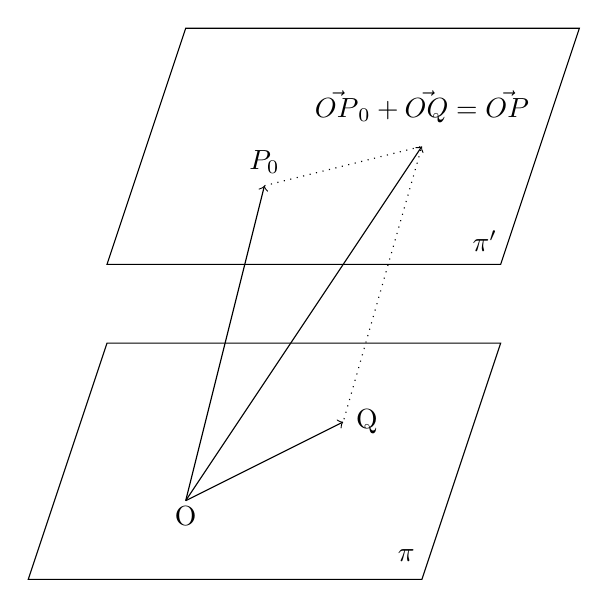
\begin{tikzpicture}
	\draw (0,0) -- (5,0) -- (6,3) -- (1,3) -- cycle;
	\draw[->] (2,1) -- (3,5);
	\draw[->]  (2,1) -- (4,2);
	\draw[->] (2,1) -- (5,5.5);
	\draw[dotted] (3,5) -- (5,5.5) -- (4,2);
	\draw (1,4) -- (6,4) -- (7,7) -- (2,7) -- cycle;
	% etichette
	\node(origine) at (2,0.8) {O};
	\node (Q) at (5,6){$\vec{OP}_0+\vec{OQ}=\vec{OP}$};
	\node (pi) at (4.8,.3) {$\pi$};
	\node (pipr) at (5.8,4.3) {$\pi^\prime$};
	\node (P0) at (3,5.3) {$P_0$};
	\node (Q) at (4.3,2) {Q};
\end{tikzpicture}
  \caption{Dimostrazione grafica di $S=\vec{OP}_0+W$}
  \label{fig:OP0piuW}
\end{figure}

Con un ragionamento e un disegno analogo, si può vedere che l'insieme dei vettori $\vec{OP}$ il cui
secondo estremo $P$ sta su una retta non passante per $O$ è un sottospazio affine.\\
Ispirati da questi esempi, si dice spesso che un sottospazio affine è \textit{il traslato di un
  sottospazio vettoriale}.

\section{Qualche applicazione geometrica}
\label{sec:qualcheappgeo}

È il caso di esporre alcuni problemi geometrici che possono essere risolti grazie al procedimento
di riduzione a gradini e al concetto di rango.\\
Ad esempio, considerando due rette $r$ e $r^\prime$ di equazioni cartesiane
\begin{eqnarray}
  \label{eq:qualcheappgeo1}
  r:
  \begin{cases}
    x+y+z=2\\
    2x-y+z=5
  \end{cases}, & r^\prime:
  \begin{cases}
    x-y-2z=-2\\
    x+3y+2z=2
  \end{cases}
\end{eqnarray}
e supponendo di velor determinare se ese hanno punti in comune. Dal momento che i punti di una retta
espressa in equazioni cartesiane sono proprio le soluzioni del sistema formato dalle due equazioni,
i punti comuni alle due rette sono dati dalle soluzioni comuni a tutte e quattro le equazioni delle
due rette, ovvero le soluzioni del sistema
\begin{equation}
  \label{eq:qualcheappgeo2}
  r:
  \begin{cases}
    x+y+x=2\\
    2x-y+z=5\\
    x-y-2z=-2\\
    x+3y+2z=2
  \end{cases}
\end{equation}
Riducendo la matrice completa si ottine
\begin{eqnarray*}
  \left(
  \begin{array}[ht!]{ccc|c}
    1 & 1 & 1 & 2\\
    2 & -1 & 1 & 5\\
    1 & -1 & -2 & -2\\
    1 & 3 & 2 & 2
  \end{array}\right)
  \overrightarrow{
  \begin{matrix}
    R_2\to R_2-2R_1\\
    R_3\to R_3-R_1\\
    R_4\to R_4-R_1
  \end{matrix}
  }\left(
  \begin{array}[ht!]{ccc|c}
    1 & 1 & 1 & 2\\
    0 & -3 & -1 & 1\\
    0 & -2 & -3 & -4\\
    0 & 2 & 1 & 0
  \end{array}\right)\\ \overrightarrow{
  \begin{matrix}
    R_3\to 3R_3-2R_2\\
    R_4\to 3R_4+2R_2
  \end{matrix}
  }\left(
  \begin{array}[ht!]{ccc|c}
    1 & 1 & 1 & 2\\
    0 & -3 & -1 & 1\\
    0 & 0 & -7 & -14\\
    0 & 0 & 1 & 2
  \end{array}\right)\overrightarrow{R_4\to7R_4+R_3}
  \left(
  \begin{array}[ht!]{ccc|c}
    1 & 1 & 1 & 2\\
    0 & -3 & -1 & 1\\
    0 & 0 & -7 & -14\\
    0 & 0 & 0 & 0
  \end{array}
  \right)
\end{eqnarray*}
Quindi il sistema è compatibile e, essendosi annullata una riga, la matrice
ha rango 3, quindi avendo 3 incognite in base a quanto detto nel Teorema \ref{teo:gauss-jordan1}
è presente solo una soluzione, viene trovata risolvendo il sistema ridotto corrispondente
\begin{equation*}
  \begin{cases}
    x+y+z=2\\
    -3y-z=1\\
    -7z=-14
  \end{cases}
\end{equation*}
Dall'ultima equazione si ottiene $z=2$, che sostituito nella seconda dà
\begin{equation*}
  -3y=z+1=2+1=3
\end{equation*}
Quindi l'unica soluzione del sistema è data dalla terna $(1,-1,2)$, che sono le coordinate
del punto in cui si incontrano le due rette.
Supponendo invece che le rette siano
\begin{eqnarray}
  \label{eq:qualcheappgeo3}
  r:
  \begin{cases}
    x+y+z=0\\
    2x+y+-z=1
  \end{cases}, & r^\prime:
                 \begin{cases}
                   2x-y=3\\
                   x+y-z=1
                 \end{cases}
\end{eqnarray}
e supponendo anche di voler determinare se esse hanno punti in comune. Come sopra, si mette insieme
le quattro equazioni e si riduce la matrice completa del sistema così ottenuto:
\begin{equation}
  \label{eq:qualcheappgeo4}
  \begin{matrix}
    \left(
    \begin{array}{ccc|c}
      1 & 1 & 2 & 0\\
      2 & 1 & -1 & 1\\
      2 & -1 & 0 & 3\\
      1 & 1 & -1 & 1
    \end{array}\right)\overrightarrow{
    \begin{matrix}
      R_2\to R_2-2R_1\\
      R_3\to R_3-2R_1\\
      R_4\to R_4-R_1
    \end{matrix}
    }\left(
    \begin{array}{ccc|c}
      1 & 1 & 1 & 0\\
      0 & -1 & -3 & 1\\
      0 & -3 & -2 & 3\\
      0 & 0 & -2 & 1
    \end{array}\right) \overrightarrow{R_3\to R_3-3R_2}\\
    \left(
    \begin{array}{ccc|c}
      1 & 1 & 1 & 0\\
      0 & -1 & -3 & 1\\
      0 & 0 & 7 & 0\\
      0 & 0 & -2 & 1
    \end{array}
    \right) \overrightarrow{R_4\to7R_4+2R_3}
    \left(\begin{array}{ccc|c}
      1 & 1 & 1 & 0\\
      0 & -1 & -3 & 1\\
      0 & 0 & 7 & 0\\
      0 & 0 & 0 & 7
    \end{array}\right)
\end{matrix}
\end{equation}
Essendo il sistema incompatibile (l'ultima riga corrisponde all'uguaglianza falsa $0=7$) è possibile
dedurre che le due rette non hanno punti in comune.\\
Ora, mentre nel piano due rette non hanno punti in comune sono neccessariamente parallele, nello spazio
tridimensionale questo non è più vero: come si vede nella seguente figura, grazie alla dimensione extra
rispetto al piano, possono trovarsi su piani paralleli e quindi non incontrarsi pur avendo la stessa
direzione.
\clearpage
\begin{figure}[ht!]
  \centering
  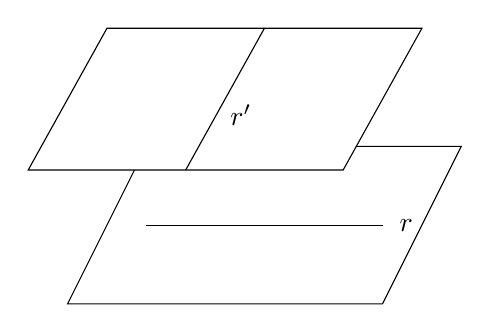
\begin{tikzpicture}
	\draw (0,0) -- (4,0) -- (5,2) -- (1,2) -- cycle;
	\draw[fill=white] (-.5,1.7) -- (3.5,1.7) -- (4.5,3.5) -- (.5,3.5) -- cycle;
	\draw (1,1) -- (4,1);
	\draw (1.5,1.7) -- (2.5,3.5);

	\node (r) at (4.3,1) {$r$};
	\node (rp) at (2.2,2.4) {$r^\prime$};
\end{tikzpicture}
  \caption{Rette su piani paralleli}
  \label{fig:rettpar}
\end{figure}

In tal caso si dice che le rette sono \textit{sghembe}. Adesso è il caso di vedere come sia possibile
determinare se le rette sono \textit{sghembe} oppure \texttt{parallele} senza fare ulteriori conti, 
ma sfruttando la riduzione già svolta. Infatti, le due rette che non hanno punti in comune sono
parallele se e solo se quando le si trasla parallelamente a se stesse sull'origine esse risultano
coincidere (ovvero hanno infiniti punti in comune), mentre sono sghembe se e solo se quando le
si trasla parallelamente a se stesse sull'origine esse hanno in comune un solo punto, l'origine stessa:
\begin{figure}[ht!]
  \centering
  \begin{tikzpicture}
	\draw (1,1) -- (4,4);
	\draw (2,1) -- (5,4);
	\draw (3,1) -- (6,4);

\end{tikzpicture}
  \caption{Differenza tra parallele e sghembe}
  \label{fig:retteparesghembe}
\end{figure}
adesso è il caso di trattare il problema di capire se le due rette hanno
la stessa direzione nel problema di determinare un'intersezione (tra le
rette traslate). Ora, per traslare una retta espressa in equazioni
cartesiane, parallelamente a se stessa, basta modificare i termini noti
delle equazioni lasciando invariati i primi membri\footnote{Infatti,
  modificando solo il noto dell'equazione $ax+by+cz=d$ di un piano si
  ottiene un piano parallelo in quanto non si avrà cambiato la normale al
  piano, data dalla terna $(a,b,c)$. Poiché una retta è intersezione di due
  piani, modificando i termini noti delle due equazioni si sta muovendo
  parallelamente a se stessi i piani e quindi muovendo parallamente a se
  stessa la retta.}: in particolare, si ottiene la traslazione sull'origine
se si va apporre i termini noti uguali a zero (in quanto in tal caso le
le equazioni risultato soddisfatte dalla terna $x=0,y=0,z=0$, che sono le
coordinate dell'origine, il che significa che la retta traslata è
proprio quella che passa per l'origine).
Nel caso delle equazioni delle due rette $r$ e $r^\prime$ data da (\ref{eq:qualcheappgeo3}), le rette
trasla sull'origine sono rappresentate dalle equazioni
\begin{eqnarray}
  \label{eq:eq:qualcheappgeo5}
  \begin{cases}
    x+y+z=0\\
    2x+y-z=0
  \end{cases}, &
                 \begin{cases}
                   2x+y=0\\
                   x+y+z=0
                 \end{cases}
\end{eqnarray}
Per determinare se tali rette traslate hanno infiniti punti in comune o uno solo, ovvero come visto
sopra, se le rette di partenza erano rispettivamente parallele o sghembe, bisogna risolvere il sistema
che si ottiene mettendo insieme le quattro equazioni,
\begin{equation*}
  \begin{cases}
    x+y+z=0\\
    2x+y-z=0\\
    2x+y=0\\
    x+y+z=0
  \end{cases},
\end{equation*}
che ha come matrice associata
\begin{equation*}
  \left(
    \begin{array}{ccc|c}
      1 &  1 &  1 & 0\\
      2 &  1 & -1 & 0\\
      2 & -1 &  0 & 0\\
      1 &  1 & -1 & 0
    \end{array}
  \right)
\end{equation*}
Ora, per ridurre a gradini questa matrice verranno applicato esattamente le stesse operazioni usate
per ridurre la (\ref{eq:qualcheappgeo4}), che differisce da essa solo per il fatto di avere tutti i
termini noti uguali a zero: l'unica differenza sarà che i termini noti rimarranno sempre nulli qualunque
operazione elementare è necessario applicare, e quindi, senza dover riscrivere il processo prima visto,
sapendo che si arriverà alla stessa matrice ridotta ma con l'ultima colonna (quuella dei termini noti)
tutta nulla, ovvero
\begin{equation*}
  \left(
    \begin{array}{ccc|c}
      1 &  1 &  1 & 0\\
      0 & -1 & -3 & 0\\
      0 &  0 &  7 & 0\\
      0 &  0 &  0 & 0
    \end{array}
  \right)
\end{equation*}
Guardando questa matrice, che rappresenta ora un sistema compatibile con 3 incognite e rango 3, si
conclude che traslando le rette sull'origine si avrà solo una soluzione (l'origine stessa) e quindi le
rette di partenza non erano parallele.\\
Adesso, è il caso di vedere cosa potrebbe capitare se le rette sono pallele, prendendo il seguente
esempio
\begin{eqnarray}
  \label{eq:qualcheappgeo6}
  r:
  \begin{cases}
    x+y+z=1\\
    x-y+2z=0
  \end{cases}, & r^\prime:
                 \begin{cases}
                   2x+3z=3\\
                   x+3y=-3
                 \end{cases}
\end{eqnarray}
Allo scopo di controllare se le rette hanno punti in comune, come visto nel caso precedente, è
necessario andare a costituire un singolo sistema composto dai due sistemi di partenza $r$ e $r^\prime$,
il risultato sarà il seguente:
\begin{equation*}
    r_{tot}:
  \begin{cases}
    x+y+z=1\\
    x-y+2z=0\\
    2x+3z=3\\
    x+3y=-3
  \end{cases}
\end{equation*}
Da questo è possibile dedurre che la matrice completa di questo sistema sarà:
\begin{equation}
  \label{eq:qualcheappgeo7}
\begin{matrix}
  \left(
    \begin{array}{ccc|c}
      1 & 1 & 1 & 1\\
      1 & -1 & 2 & 0\\
      2 & 0 & 3 & 3\\
      1 & 3 & 0 & -3
    \end{array}\right)
  \overrightarrow{
     \begin{matrix}
       R_2\to R_2-R_1\\
       R_3\to R_3-2R_1\\
       R_4\to R_4-R_1
     \end{matrix}
   }
 \left(
   \begin{array}{ccc|c}
     1 & 1 & 1 & 1 \\
     1  & -2 & 1 & -1 \\
     0  & -2 & 1 & 1 \\
     0 & 2 & -1 & -4
   \end{array}
 \right) \overrightarrow{
   \begin{matrix}
     R_3\to R_3-R_2\\
     R_4\to R_4+R_2
   \end{matrix}
}\\
\left(
  \begin{array}{ccc|c}
    1 & 1 & 1 & 1 \\
    1 & -2 & 1 & -1 \\
    0 & 0 & 0 & 2 \\
    0 & 0 & 0 & -5
  \end{array}
  \right)\overrightarrow{R_4\to 2R_4+5R_3}\left(
  \begin{array}{ccc|c}
    1 & 1 & 1 & 1 \\
    1 & -2 & 1 & -1\\
    0 & 0 & 0 & 2\\
    0 & 0 & 0 & 0
  \end{array}\right)
  \end{matrix}
\end{equation}
COme si vede, da una partte le rette non hanno punti in comune in quanto la teza riga corrisponde
all'uguaglianza falsa $0 = 2$; dall'altra parte, il sistema formato dalle due rette traslate
sull'origine, ovvero con termini noti nulli, avrebbe come matrice ridotta la stessa matrice ottenuta
ora ma con l'ultima colonna composta da zeri, ovvero
\begin{equation*}
  \left(
    \begin{array}{ccc|c}
      1 & 1 & 1 & 0 \\
      1 & -2 & 1 & 0\\
      0 & 0 & 0 & 0\\
      0 & 0 & 0 & 0
    \end{array}
  \right)
\end{equation*}
Che rappresenta la matrice di un sistema ridotto compatibile con 3 incognite e rango 2, quindi infinite
soluzioni: questo rsignifica che le due rette, traslate sull'origine, hanno infiniti punti in comune,
ovvero coincidono, e quindi le due rette di partenza, prima della traslazione, erano parallele.
\begin{oss}
  \label{oss:qualcheappgeo3}
Per rette date in equazioni parametriche verificate se esse sono parallele o meno è immediata, in quento
come già definito in precedenza, nel equazioni parametriche
\begin{equation*}
  \begin{cases}
    x=x_0+lt\\
    y=y_0+mt\\
    z=z_0+nt
  \end{cases}
\end{equation*}
un vettore che rappresenta la direzione della retta è dato dalla terna $(l,m,n)$ dei coefficenti di
$t$ (questo è scrivibile maticamente anche in forma $\frac{l}{l^\prime}=\frac{m}{m^\prime}=
\frac{n}{n^\prime}$): basta quindi confrontare i due vettori così ottenuti per ognuna delle due rette,
che avranno la stessa direzione se tali vettori sono proporzionali. Nel caso in cui le rette siano date
in equazioni cartesiane, si può passare alle parametriche semplicmente risolvendo i sistemi dati dalle
cartesiane stesse. Ad esempio, per le rette viste sopra in (\ref{eq:qualcheappgeo6}), riducendo la
matrice completa delle cartesiane di $r$ si ottiene
\begin{equation*}
  \left(
    \begin{array}{ccc|c}
      1 & 1 & 1 & 1 \\
      1 & -1 & 2 & 0
    \end{array}
  \right)\overrightarrow{R_2\to R_2-R_1}
\left(
  \begin{array}{ccc|c}
    1 & 1 & 1 & 1 \\
      0 & -2 & 1 & -1
  \end{array}
\right)
\end{equation*}
ovvero il sistema ridotto $
\begin{cases}
  x+y+z=1\\
  -2y+z=-1
\end{cases}
$, da cui ponendo $z=t$ si ricava $-2y=-1-t$ (ovvero $y=\frac{1}{2}+\frac{1}{2}t$) e $x=1-y-z=
1-\left(\frac{1}{2}+\frac{1}{2}t\right)-t=\frac{1}{2}-\frac{3}{2}t$ quindi $r$ ha equazioni parametriche
  \begin{equation}
    \label{eq:qualcheappgeo8}
    \begin{cases}
      x=\frac{1}{2}-\frac{3}{2}t\\
      y=\frac{1}{2}+\frac{1}{2}t\\
      z=t
    \end{cases}
  \end{equation}
  Analogamente, riduzione la matrice completa delle cartesiane di $r^\prime$ ottenendo
  \begin{equation*}
    \left(
      \begin{array}{ccc|c}
        2 & 0 & 3 & 3 \\
        1 & 3 & 0 & -3
      \end{array}
    \right)\overrightarrow{R_2\to2R_2-R_1}\left(
      \begin{array}{ccc|c}
        2 & 0 & 3 & 1 \\
        0 & 6 & -3 & -9
      \end{array}
    \right)
  \end{equation*}
  ovvero il sistema ridotto $
  \begin{cases}
    2x+3z=3\\
    6y-3z=-9
  \end{cases}
  $, da cui ponendo $z = t$ si ricava $6y=-9+3t$ (ovvero $-\frac{3}{2}+\frac{1}{2}t$) e $2x=3-3z=3-3t$,
  ovvero $x=\frac{3}{2}-\frac{3}{2}t$: quindi $r$ ha equazioni parametriche
  \begin{equation}
    \label{eq:qualcheappgeo9}
    \begin{cases}
      x=\frac{3}{2}-\frac{3}{2}t\\
      y=-\frac{3}{2}+\frac{1}{2}t\\
      z=t
    \end{cases}
  \end{equation}
  Confrontando i coefficienti di $t$ nelle parametriche (\ref{eq:qualcheappgeo8}) e
  (\ref{eq:qualcheappgeo9}), si vede che le rette hanno entrambe direzione rappresentata dal vettore
  di coordinate $\left(-\frac{3}{2},\frac{1}{2},1\right)$, e quindi sono parallele\footnote{Si
    noti che le rette hanno la stessa direzione, che non esclude il caso in cui esse siano parallele
    coincidenti, ovvero che le equazioni cartesiane date rappresentassero in realtà la stessa retta.}.
\end{oss}
\begin{oss}
  \label{oss:qualcheappgeo4}
  Nel caso in cui si ovglia fare il passaggio inverso, ovvero passare da parametriche a cartesiane, nel
  caso della retta basta ricavare il parametro $t$ da una delle espressioni che compongono le
  parametriche e sostituirlo nelle altre. Ad esempio, se la retta ha equazioni parametriche
  \begin{equation*}
    \begin{cases}
      x=1-t\\
      y=2+t\\
      z=1-3t
    \end{cases}
  \end{equation*}
  si può ricavare $t=1-x$ dalla prima che, sostituita nelle altre, da $y=2+(1-x)=3-x$ e
  $1-3 (1-x)=-2+3x$. allora è anche possibile affermare che la retta ha equazioni cartesiane
  \begin{equation*}
    \begin{cases}
      x=1+t+s\\
      y=2+t-s\\
      z=3-2t-s
    \end{cases}
  \end{equation*}
  si può ricavare $t=x-1-s$ dalla prima che, sostituita nelle altre, dà $y=2+(x-1-s)-s=1+x-2s$ e
  $z=3-2(x-1-s)-s=5-2x+s$; ricavano poi $s$ da questa seconda espressione, ovvero $s=z+2x+s$; ricavano
  poi $s$ da questa seconda espressione, ovvero $s=z+2x-5$, è possibile sostituire nell'altra
  ottenendo $y=1+x-2(z+2x-5)=11-3x-2z$, ovvero $3x+y+2z=11$, che è l'equazione cartesiana del piano.
  Nel capicolo successivo verrà illustrato un metodo più elegante e efficiente per arrivare allo stesso
  risultato.\\
  Un altro problema geometrico che può essere risolto con l'aiuto delle tecniche viste a proposito della
  risoluzione dei sistemi è il seguente: supponendo di avere una retta data in equazioni cartesiane
  \begin{eqnarray}
    \label{eq:qualcheappgeo10}
    \begin{cases}
      Ax+By+Cz=D\\
      A^\prime x+B^\prime y+C^\prime z =D^\prime
    \end{cases}
  \end{eqnarray}
  Come visto nel capitolo precedente quando si tratta di ricavare tali equazioni, la
  (\ref{eq:qualcheappgeo10}) sta semplicemente dicendo che la retta data è intersezione del piano dato
  dall'equazione cartesiana $Ax+By+Cz=D$ e dal piano di equazione cartesiana $Ax+By+Cz=D$ e dal piano
  di equazione cartesiana $A^\prime x+B^\prime y+C^\prime z =D^\prime$: le due equazioni che compongono
  le cartesiane sono quindi le equazioni di due particolari piani che contengono la retta.
  Per determinare tutti i piani che contengiono la retta, bisogna esporre la seguente
\end{oss}
\begin{prop}
  \label{prop:qualcheappgeo4}
  La generica equazione cartesiana del piano che contiene la retta (\ref{eq:qualcheappgeo10}) è data
  da
  \begin{equation}
    \label{eq:qualcheappgeo11}
    \alpha (Ax+By+Cz-D)+\beta (A^\prime x +B^\prime y + C^\prime-D^\prime)=0
  \end{equation}
  al variare di $\alpha,\beta\in \mathds{R}$.
\end{prop}
\begin{proof}
  Bisogna iniziare con l'osservare che se un piano ha equazione della forma (\ref{eq:qualcheappgeo11}),
  allora esso contiene la reta. Infatti, dire che una retta è contenuta in un piano significa che se
  un punto appartiene anche al piano: ma se un punto appartiene alla retta, allora le sue coordinate
  $(x,y,z)$ soddisfano entrambe le equazioni $Ax+By+Cz=D$ e $A^\prime x+B^\prime+C^\prime z=D^\prime$ della
  retta, e quindi
  \begin{eqnarray*}
    \alpha(Ax+By+Cz-D)+\beta(A^\prime x+B^\prime y+C^\prime z-D^\prime) = \alpha \cdot 0+\beta \cdot 0=0
  \end{eqnarray*}
  ovvero $(x,y,z)$ soddisfa anche l'equazione (\ref{eq:qualcheappgeo11}), cioè il punto appartiene al
  piano rappresentato da tale equazione. Questo dimostra che, per ogni $\alpha, \beta\in \mathds{R}$,
  l'equazione (\ref{eq:qualcheappgeo11}) rappresenta un piano che contiene la retta.
  Viceversa, bisogna essere sicuri che qualche paiano che contenga la retta può essere rappresentato
  nella forma (\ref{eq:qualcheappgeo11}). Per vederlo, bisogna osservere che un generico piano di
  equazione $A^{\prime\prime}x+B^{\prime\prime}y+C^{\prime\prime}=D^{\prime\prime}$ contiene tutta la
  retta sta anche sul piano, ovvero se e solo se ogni terna che soddisfa le equazioni
  $Ax+By+Cz=D$ e $A^{\prime}x+B^{\prime}y+C^{\prime}=D^{\prime}$ soddisfa automaticamente anche
  l'equazione $A^{\prime\prime}x+B^{\prime\prime}y+C^{\prime\prime}=D^{\prime\prime}$ del piano.
  In altre parole, nel sistema
  \begin{eqnarray*}
    \begin{cases}
      Ax+By+Cz=B\\
      A^{\prime}x+B^{\prime}y+C^{\prime}=D^{\prime}\\
      A^{\prime\prime}x+B^{\prime\prime}y+C^{\prime\prime}=D^{\prime\prime}
    \end{cases}
  \end{eqnarray*}
  che si ottiene mettendo insieme tutte le cartesiane, la terza equazione è superfluo ovvero dipendente
  dalle altre. A livello della matrice completa
  \begin{eqnarray*}
    \begin{vmatrix}
      A & B & C & D\\
      A^\prime & B^\prime & C^\prime & D^\prime\\
      A^{\prime\prime} & B^{\prime\prime} & C^{\prime\prime} & D^{\prime\prime}
    \end{vmatrix}
  \end{eqnarray*}
  questo si traduce nel fatto che la terza riga deve essere combinazione lineare delle altre due,
  ovvero devono esistere $\alpha,\beta\in\mathds{R}$ tali che
  \begin{eqnarray*}
    \begin{vmatrix}
      A^{\prime\prime} & B^{\prime\prime} & C^{\prime\prime} & D^{\prime\prime}
    \end{vmatrix}=\alpha
    \begin{vmatrix}
      A & B & C & D
    \end{vmatrix} +\beta
    \begin{vmatrix}
      A^\prime & B^\prime & C^\prime & D^\prime
    \end{vmatrix}
  \end{eqnarray*}
  ovvero
  \begin{eqnarray*}
    \begin{matrix}
      A^{\prime\prime}=\alpha A +\beta A^\prime, & B^{\prime\prime}=\alpha B+\beta B^\prime,
      & C^{\prime\prime} =\alpha C + \beta C^\prime, & D^{\prime\prime}=\alpha D+\beta D^\prime
    \end{matrix}
  \end{eqnarray*}
  Quindi l'equazione $A^{\prime\prime}x+B^{\prime\prime}y+C^{\prime\prime}=D^{\prime\prime}$ si riscrive
  \begin{eqnarray*}
    (\alpha A+\beta A^\prime)x+(\alpha B+\beta B^\prime)y+(\alpha C+\beta C^\prime)z=\alpha D + \beta
    D^\prime
  \end{eqnarray*}
  che, si vede facilmente svolgendo i conti e confrontando, equivale proprio alla
  (\ref{eq:qualcheappgeo11}).
\end{proof}
\begin{es}
  \label{es:qualcheappgeo1}
  Data la retta
  \begin{equation*}
    r:
    \begin{cases}
      x+y+z=1\\
      x-y+2z=0
    \end{cases}
  \end{equation*}
  si determini il piano $\pi$ che contiene $r$ e passa per il punto $P_0$ di coordinate $(1,1,1)$.
  Determinando prima tutti i piani che contengono $r$, che secondo la Proposizione
  \ref{prop:qualcheappgeo4} sono dati al variare di $\alpha,\beta\in \mathds{R}$ dall'equazione
  \begin{equation}
    \label{eq:qualcheappgeo12}
    \alpha(x+y+z-1) +\beta(x-y+2z)=0.
  \end{equation}
  da cui $\alpha=-\beta$. Sostituendo questa relazione nella (\ref{es:qualcheappgeo1}), si ottiene
  \begin{equation*}
    -\beta(x+y+z-1)+\beta(x-y+2z)=0
  \end{equation*}
  ovvero, svolgendo i calcli,
  \begin{equation*}
    -2y+z+1=0.
  \end{equation*}
  Al variare del parametro $\beta$, queste equazioni rappresentano tutte lo stesso piano (il piano
  $\pi$ cercato) in quanto si tratta di equazioni proporzionali, tutte equivalenti: dividendo per
  il parametro $\beta$ (o, equivalentemente, scegliendo per esempio $\beta=1$), possiamo allora scrivere
  che $\pi$ ha equazione cartesiana
  \begin{equation*}
    -2y+z+1=0.
  \end{equation*}
  Se, invece del passaggio per il punto, nel caso in cui si impone per esempio che il piano, oltre a
  contenere $r$, fosse parallelo a un altro piano, ad esempio quello di equazione cartesiana
  $x+2y+3z=-1$, bisogna procesere come segue. Come visto nel capitolo precedente, due piani
  $Ax+By+Cz=D$ e $A^\prime x+B^\prime y+C^\prime z=D^\prime$ sono paralleli se e solo se le terne $(A,B,C)$
  e $(A^\prime,B^\prime,C^{\prime})$ sono proporzionali, in quanto rappresentano le coordinate di vettori
  normali (perpendicolari) ai piani. In realtà, paiché c'è la libertà di moltiplicare l'equazione di un
  piano per qualunque coefficiente senza che il piano venga modificato, si può sempre far che sia
  $(A,B,C)=(A^\prime,B^\prime,C^\prime)$. Allora, poiché svolgendo i calcoli nella
  (\ref{eq:qualcheappgeo12}), il generico piano che contiene $r$ è della forma
  \begin{equation}
    \label{eq:qualcheappgeo13}
    (\alpha+\beta)x+(\alpha-\beta)y+(\alpha+2\beta)z-\alpha = 0,
  \end{equation}
  la condizione di parallelism,o tra questo piano e il piano di equazione $x+2y+3z=-1$ è
  \begin{eqnarray*}
    (\alpha+\beta,\alpha-\beta,\alpha+2\beta)=(1,2,3)
  \end{eqnarray*}
  ovvero, trasponendo questo modello in forma sistemica ordinata:
  \begin{eqnarray*}
    \begin{cases}
      \alpha+\beta=1\\
      \alpha-\beta=2\\
      \alpha-2\beta=3
    \end{cases}
  \end{eqnarray*}
  Per trovare il piano dato, basta quindi risolvere tale sistema e
  sostituire valori di $\alpha$ e $\beta$ trovati nella equazione
  (\ref{eq:qualcheappgeo13}). In questo caso, si vede riducendo a gradini
  la sua matrice completa
  \begin{eqnarray*}
    \left(
    \begin{array}{cc|c}
      1 & 1 & 1 \\
      1&-1&2 \\
      1 & 2 &3
    \end{array}
    \right)\overrightarrow{
    \begin{matrix}
      R_1\to R_2-R_1\\
      R_3\to R_3-R_1
    \end{matrix}
    }\left(
    \begin{array}{cc|c}
      1 & 1 & 1 \\
      0 &-2&1 \\
      0&1&2
    \end{array}
    \right)
    \overrightarrow{R_3\to R_3+R_2}
    \left(
    \begin{array}{cc|c}
      1&1&1 \\
      0&-2&1 \\
      0&0&5
    \end{array}\right)
  \end{eqnarray*}
  il sistema è incompatible e quindi la condizione di parallelismo non
  può essere soddisfatta: tra i piani che contengono la retta $r$, non
  ne esiste nessuno che è parallelo al piano dato.
\end{es}
\begin{es}
  Date le due rette
  \begin{eqnarray*}
    r_1:
    \begin{cases}
      x+y+z=3\\
      x-2y+z=0
    \end{cases}, & r_2:
                   \begin{cases}
                     2x+y-z=2\\
                     x-y-z=-1
                   \end{cases}
  \end{eqnarray*}
  bisogna determinare, se esiste, il piano che le contiene.
  Come fatto precedente, il generico piano che contiene $r_1$ ha
  equazione
  \begin{eqnarray*}
    \alpha_1(x+y+z-3)+\beta_1(x-2y+z)=0
  \end{eqnarray*}
  ovvero, espresso in altra forma:
  \begin{equation}
    \label{eq:qualcheappgeo14}
    (\alpha_1+\beta_1)x+(\alpha_1-2B_1)y+(\alpha_1+\beta_1)z-3\alpha_1=0
  \end{equation}
  mentre il generico piano che contiene $r_2$ ha equazione
  \begin{eqnarray*}
    \alpha_2(2x+y+z-2)+\beta(x-y-z+1)=0
  \end{eqnarray*}
  ovvero
  \begin{equation}
    \label{eq:qualcheappgeo15}
    (2\alpha_2+\beta_2)x+(\alpha_2-\beta_2)y+(-2\alpha_2+\beta_2)z
    +(-2\alpha_2+\beta_2)=0.
  \end{equation}
  Per trovare, se siste, il piano che contiene entrambe le rette basta
  vedere se osistono valori di $\alpha_1,\beta_1,\alpha_2,\beta_2$ tali
  che la (\ref{eq:qualcheappgeo14}) e la (\ref{eq:qualcheappgeo15}) sono
  uguali: uguagliando i coeffcienti di $x,y,z$ e il temine noto in tali
  equazioni si ottiene
  \begin{eqnarray*}
    \begin{cases}
      \alpha_1+\beta_1=2\alpha_2+\beta_2\\
      \alpha_1-2\beta_1=\alpha_2-\beta_2\\
      \alpha_1+\beta_1=-\alpha_2-\beta_2\\
      -3\alpha_1=-1\alpha_2+\beta_2
    \end{cases}
  \end{eqnarray*}
  ovvero il sistema omogeneo di 4 equazioni in 4 incognite
  \begin{eqnarray*}
    \begin{cases}
      \alpha_1+\beta_1=2\alpha_2+\beta_2=0\\
      \alpha_1-2\beta_1=\alpha_2-\beta_2=0\\
      \alpha_1+\beta_1=-\alpha_2-\beta_2=0\\
      -3\alpha_1=-1\alpha_2+\beta_2=0
    \end{cases}
  \end{eqnarray*}
  Tale sistema ha sicuramente sempre la soluzione $\alpha_1=\beta_1
  =\alpha_2=\beta_2=0$, ma se si sostituiscono tali valori nella
  (\ref{eq:qualcheappgeo14}) e la (\ref{eq:qualcheappgeo15}) ottenendo
  $0=0$, che non è l'equazione di un piano: quindi per l'esistenza del
  piano che contiene entrambe le rette deve esistere una soluzione non
  nulla di tale sistema. Riducendo a gradini la sua matrice dei
  coefficienti si trova
  \begin{eqnarray*}
    \begin{bmatrix}
      1 & 1 & -2 & -1\\
      1 & -2 & -1 & 1\\
      1 & 1 & 1 & 1\\
      -3 & 0 & 2 & -1
    \end{bmatrix}\overrightarrow{
    \begin{matrix}
      R_2\to R_2-R_1\\
      R_1\to R_3-R_1\\
      R_4\to R_4-3R_1
    \end{matrix}
    }
    \begin{bmatrix}
      1 & 1 & -2 & -1\\
      0 & -3 & 1 & 2\\
      0 & 0 & 3 & 2\\
      0 & 3 & -4 & -4
    \end{bmatrix}
    \overrightarrow{R_4\to R_4+R_2}
    \begin{bmatrix}
      1 & 1 & -2 & -1\\
      0 & -3 & 1 & 2\\
      0 & 0 & 3 & 2\\
      0 & 0 & -3 & -2
    \end{bmatrix}\\\overrightarrow{R_4\to R_4+R_3}
    \begin{bmatrix}
      1 & 1 & -2 & -1\\
      0 & -3 & 1 & 2 \\
      0 & 0 & 3 & 2\\
      0 & 0 & 0 & 0
    \end{bmatrix}
  \end{eqnarray*}
  Poiché la matrice ha rango 3 il sistema ha sicuramente altre soluzioni
  oltre alla 4-uple nulla $(0,0,0,0)$, quindi esiste il piano che contiene
  le rette. Per trovarlo, basta risolvere il sistema, che ridotto
  precedentemente alla forma equivalente
  \begin{eqnarray*}
    \begin{cases}
      \alpha_1+\beta_1-2\alpha_2-\beta_2=0\\
      -3\beta_1+\alpha_2+3\beta_2=0\\
      3\alpha_2+2\beta_2=0
    \end{cases}
  \end{eqnarray*}
  Però non è necessario determinare completamente la soluzione del
  sistema: infatti, l'ultima equazione non nulla dà il valore di
  $\alpha_2$ (in funzione di $\beta_2$), mentre le prime due i valori
  $\alpha_1$ e $\beta_1$ (sempre in forma di $\beta_2$): se si sostituisce
  i valori $\alpha_1$ e $\beta_1$ così trovati nella
  (\ref{eq:qualcheappgeo14}) o quello di $\alpha$ nella
  (\ref{eq:qualcheappgeo15}) ottenendo lo stesso piano (il sistema
  esprimendo porprio la condizione che i due piani sono uguali), quindi
  per trovarlo basta determinare solo $\alpha_2$ dall'ultima equazione non
  nulle $2\alpha_2+2\beta_2=0$ senza dover risolvere le altre due.
  Questa equazione dà $\alpha_2=\frac{2}{3}\beta_2$ che sostituita nella
  (\ref{eq:qualcheappgeo15}) da
  \begin{eqnarray*}
    \left(-\frac{4}{3}\beta_2+\beta_2\right)x+\left(-\frac{2}{3}\beta_2
    -\beta_2\right)y+\left(\frac{2}{3}\beta_2-\beta_2\right)z+
    \left(\frac{4}{3}\beta_2+\beta_2\right)=0
  \end{eqnarray*}
  ovvero
  \begin{eqnarray*}
    -\frac{1}{3}\beta_2x+\frac{5}{3}\beta_2y-\frac{1}{3}\beta_2z+
    \frac{7}{3}\beta_2=0
  \end{eqnarray*}
  Dividendo per $\beta_2$ e moltiplicando per $-3$ si ottiene infine
  \begin{eqnarray*}
    x+5y+z-7=0
  \end{eqnarray*}
  che è l'equazione del piano cercato.
\end{es}
Il procedimento di riduzione a gradini è uno strumento non solo per
risolvere un sistema ma più in generale per scoprire se delle $n$-uple
sono linearmente indipendenti e in caso negativo, per individuare le
$n$-uple che sono combinazione delle altre. A sua volta questo contente
di determinare se sono indipendenti i vettori in un qualunque spazio
vettoriale: infatti, basta fissare una base, rappresentare i vettori
mediante le $n$-uple delle loro coordinate e poi controllare se sono
indipendenti tali $n$-uple mediante una semplice riduzione a gradini.
\begin{es}
  Fissata una base $\vec{OP}_1,\vec{OP}_2,\vec{OP}_3$ dello spazio
  tridimensionale dei vettori applicati $V_O^3$, si dica se i tre vettori
  applicati
  \begin{eqnarray*}
    v_1=\vec{OP}_1+\vec{OP}_2+\vec{OP}_3\\
    v_2=3\vec{OP}_1+4\vec{OP}_2+5\vec{OP}_3\\
    v_3=-\vec{OP}_1+2\vec{OP}_2+5\vec{OP}_3
  \end{eqnarray*}
  formano ancora una base.
  Tre vettori in uno spazio di dimensione 3 formano una base se e solo se
  sono indipendenti: per determinare l'indipendenza di $v_1,v_2,v_3$ basta
  considerare le terne $(1,2,3),(3,4,5),(-1,2,5)$ delle loro coordinate
  rispetto alla base di partenza $OP_1,OP_2,OP_3$ e determinare
  equivalentamente se esse sono indipendenti in $\mathds{R}$.
  \clearpage
  Costruendo la matrie che ha tali terne come righe
  \begin{eqnarray*}
    \begin{bmatrix}
      1 & 2 & 3\\
      3 & 4 & 5\\
      -1 & 2 & 5
    \end{bmatrix}
  \end{eqnarray*}
  e effetuando una riduzione a gradini:
  \begin{eqnarray*}
    \begin{bmatrix}
      1 & 2 & 3\\
      3 & 4 & 5\\
      -1 & 2 & 5
    \end{bmatrix}\overrightarrow{
    \begin{matrix}
      R_2\to R_2-3R_1\\
      R_3\to R_4+R_1
    \end{matrix}
    }
    \begin{bmatrix}
      1 & 2 & 3\\
      0 & -2 & -4\\
      0 & 4 & 8
    \end{bmatrix}
    \overrightarrow{R_3\to R_3+2R_2}
    \begin{bmatrix}
      1 & 2 & 3\\
      0 & -2 & -4\\
      0 & 0 & 0
    \end{bmatrix}
  \end{eqnarray*}
  Essendosi annullata la terza riga, significa che questa era
  combinazione delle prime due: quindi le tre terne non sono indipendenti
  e non lo sono neanche i vettori applicati $v_1,v_2,v_3$ da esse
  rappresentate (tali vettori giacevano quindi su uno stesso piano).
\end{es}

\section{Due integrazioni sul determinante}
\label{sec:dueintdet}

\subsection{Complanarità di rette in parametriche}
\label{sec:comdiretteinparametriche}

Siano $r$ e $r^\prime$ due rette, date in equazioni parametriche
\begin{eqnarray}
  \label{eq:dueintdet1}
  r:
  \begin{cases}
    x=x_0+at\\
    y=y_0+bt\\
    z=z_0+ct
  \end{cases}, & r^\prime:
                 \begin{cases}
                   x=x_0^\prime+a^\prime t\\
                   y=y^\prime_0+b^\prime t\\
                   z=z_0^\prime+c^\prime t
                 \end{cases}
\end{eqnarray}
Allora $r$ e $r^\prime$ sono complanari se e solo se
\begin{eqnarray}
  \label{eq:dueintdet2}
  \det
  \begin{bmatrix}
    x_0-x_0^\prime & y_0-y_0^\prime& z_0-z_0^\prime\\
    a & b & c\\
    a^\prime & b^\prime & c^\prime
  \end{bmatrix}=0
\end{eqnarray}
Infatti, due rette sono complanari solo se sono o parallele o incidenti
in un punto: nel caso in cui esse siano parallele, i loro vettori
direttori $v=(a,b,c)$ e $v^\prime=(a^\prime, b^\prime,
c^\prime)$\footnote{Che si vedono dai coefficienti di $t$ nelle
  parametriche} sono proporzionali, e quindi il determinante
(\ref{eq:dueintdet2}) è zero perché la seconda e la terza riga delle
matrice sono proporzionali e quindi dipendenti (e il determinante di una
matrice con le righe dipendenti, si annulla). Nel caso in cui le rette in
cui le rette siano incidenti in un punto, invece, dal momento che le
parametriche di una retta danno i punti della retta al variare del
parametro, esisteranno un valore di $t$ da sostituire nella prima delle
(\ref{eq:dueintdet1}) e un valore di $t^\prime$ da sostituire della
(\ref{eq:dueintdet1}) per i quali si ottiene lo stesso punto (quello in
comune alle due rette), ovvero per tali valori si ha
\begin{equation}
  \label{eq:dueintdet3}
  \begin{cases}
    x_0 +at=x_0^\prime+a^\prime t^\prime\\
    y_0 + bt = y_0^\prime + b^\prime t^\prime\\
    z_0+ct=z_0^\prime+c^\prime t^\prime
  \end{cases}
\end{equation}
È possibile riscrivere queste guaglianze come
\begin{eqnarray*}
  \begin{cases}
    x_0-x_0^\prime=-at+a^\prime t^\prime\\
    y_0-y_0^\prime=-bt+b^\prime t^\prime\\
    z_0-z_0^\prime=-ct+c^\prime t^\prime
  \end{cases}
\end{eqnarray*}
ovvero accorparle nella forma vettoriale
\begin{equation}
  \label{eq:dueintdet4}
  (x_0-x_0^\prime,y_0-y_0^\prime,z_0-z_0^\prime)=-(a,b,c)+t^\prime(a^\prime,
  b^\prime,c^\prime) 
\end{equation}
Qyesta uguaglianza sta allora dicendo che, nella matrice che compare nella
(\ref{eq:dueintdet2}), la prima riga è combinazione lineare delle altre
due: di nuovo, il determinante è allora zero in quanto il determinante di
una matrice con le righe dioendenti è nullo.\\
Questo conclude la dimostrazione del fatto che se le rette sono complanari
allora vale la \ref{eq:dueintdet2}. Viceversa, se il determinante si
annulla allora i casi sono due:
\begin{enumerate}
\item La seconda e la terza riga $(a,b,c)$ e $(a^\prime,b^\prime,c^\prime)$
  sono proporzionali, e le rette sono parallele, essendo tali righe i
  vettori direttori delle rette.
\item Se le rette non sono proporzionali, quando il determinante nullo e
  quindi le righe dipendenti necessariamentela prima riga
  $(x_0-x_0^\prime, y_0-y_0^\prime, z_0-z_0^\prime)$ deve essere
  combinazione lineare di $(a,b,c)$ e $(a^\prime,b^\prime,c^\prime)$:
  questo, ripetendo a ritroso i passaggi fatti per passare dalla
  (\ref{eq:dueintdet4}) alla (\ref{eq:dueintdet3}) mostra che le rette
  devono avere un punto in comune.
\end{enumerate}
  
\subsection{Regola di Sarrus}
\label{sec:regsarrus}

La regola di Sarrus è un metodo, alternativo allo svolgimento di Laplace,
per calcolare il determinante di una matrice quadrata di ordine 3
\begin{equation}
  \label{eq:dueintdet5}
  A=
  \begin{bmatrix}
    a_{11}&a_{12} & a_{13}\\
    a_{21} & a_{22} & a_{23}\\
    a_{31} & a_{32} & a_{33}
  \end{bmatrix}
\end{equation}
La regola di Sarrus funziona come segue: aggiungendo alla matrice data due
colonne ripetendo, dopo la terza, la sua prima e la sua seconda colonna:
\begin{equation}
  \label{eq:dueintdet6}
  \left[
  \begin{array}{ccccc}
    a_{11} & a_{12} & a_{13} & a_{11} & a_{12}\\
    a_{21} & a_{22} & a_{23} & a_{21} & a_{22}\\
    a_{31} & a_{32} & a_{33} & a_{31} & a_{32} 
  \end{array}\right]
\end{equation}
In questa matrice con cinque colonne è possibile mettere in evidenza tre
``diagonali''
\begin{equation}
  \label{eq:dueintdet7}
  \begin{matrix}
    \left[
    \begin{array}{ccccc}
      \mathbf{\color{blue}a_{11}} & a_{12} & a_{13} & a_{11} & a_{12}\\
      a_{21} & \mathbf{\color{blue}a_{22}} & a_{23} & a_{21} & a_{22}\\
      a_{31} & a_{32} & \mathbf{\color{blue}a_{33}} & a_{31} & a_{32} 
    \end{array}\right], & \left[
                          \begin{array}{ccccc}
                            a_{11} & \mathbf{\color{blue}a_{12}} & a_{13} & a_{11} & a_{12}\\
                            a_{21} & a_{22} & \mathbf{\color{blue} a_{23}} & a_{21} & a_{22}\\
                            a_{31} & a_{32} & a_{33} & \mathbf{\color{blue} a_{31}} & a_{32} 
                          \end{array}\right],\\ \left[
    \begin{array}{ccccc}
      a_{11} & a_{12} & \mathbf{\color{blue}a_{13}} & a_{11} & a_{12}\\
      a_{21} & a_{22} & a_{23} & \mathbf{\color{blue}a_{21}} & a_{22}\\
      a_{31} & a_{32} & a_{33} & a_{31} & \mathbf{\color{blue}a_{21}} 
    \end{array}\right],
  \end{matrix}
\end{equation}
e tre ``antidiagonali''
\begin{equation}
  \label{eq:dueintdet8}
  \begin{matrix}
    \left[
    \begin{array}{ccccc}
      a_{11} & a_{12} & \mathbf{\color{red} a_{13}} & a_{11} & a_{12}\\
      a_{21} & \mathbf{\color{red}a_{22}} & a_{23} & a_{21} & a_{22}\\
      \mathbf{\color{red}a_{31}} & a_{32} & a_{33} & a_{31} & a_{32} 
    \end{array}\right], & \left[
                          \begin{array}{ccccc}
                            a_{11} & a_{12} & a_{13}
                            & \mathbf{\color{red}a_{11}} & a_{12}\\
                            a_{21} & a_{22}
                            & \mathbf{\color{red}a_{23}} & a_{21} & a_{22}\\
                            a_{31} & \mathbf{\color{red}a_{32}} & a_{33} &  a_{31} & a_{32} 
                          \end{array}\right],\\ \left[
    \begin{array}{ccccc}
      a_{11} & a_{12} & a_{13} & a_{11} & \mathbf{\color{red} a_{12}}\\
      a_{21} & a_{22} & a_{23} & \mathbf{\color{red}a_{21}} & a_{22}\\
      a_{31} & a_{32} & \mathbf{\color{red}a_{33}} & a_{31} & a_{21} 
    \end{array}\right].
  \end{matrix}
\end{equation}
Il determinate della matrice risulta essere allora uguale al prodotto
degli elementi della prima diagonale più il prodotto degli elementi della
seconda diagonale più il prodotto degli elementi della terza diagonale,
meno il prodotto degli elementi della prima antidiagonale meno il prodotto
degli elementi della seconda antidiagonale meno il prodotto degli
elementi della terza antidiagonale:
\begin{eqnarray*}
  a_{11}a_{22}a_{33}+a_{12}a_{23}a_{31}+a_{13}a_{22}a_{32}-a_{13}a_{22}a_{31}
  -a_{11}a_{23}a_{32}-a_{12}a_{21}a_{33}
\end{eqnarray*}
Infatti, si potrebbe verificare che gli addendi di questa uguaglianza
coincidono con quelli previsti dalla definizione di determinante
mediante sommatoria e permutazioni (la regola di Sarrus dà quindi
semplicemente un modo pratico di ottenere quegli stessi addetti, con i
segni corretti, senza ricorrere alla definizione).\\
Bisogna sottolineare il fatto che la regola di Sarrus non può essere
applicata a matrici di ordine superiore a 3.
